% Options for packages loaded elsewhere
\PassOptionsToPackage{unicode}{hyperref}
\PassOptionsToPackage{hyphens}{url}
%
\documentclass[
]{article}
\usepackage{amsmath,amssymb}
\usepackage{iftex}
\ifPDFTeX
  \usepackage[T1]{fontenc}
  \usepackage[utf8]{inputenc}
  \usepackage{textcomp} % provide euro and other symbols
\else % if luatex or xetex
  \usepackage{unicode-math} % this also loads fontspec
  \defaultfontfeatures{Scale=MatchLowercase}
  \defaultfontfeatures[\rmfamily]{Ligatures=TeX,Scale=1}
\fi
\usepackage{lmodern}
\ifPDFTeX\else
  % xetex/luatex font selection
\fi
% Use upquote if available, for straight quotes in verbatim environments
\IfFileExists{upquote.sty}{\usepackage{upquote}}{}
\IfFileExists{microtype.sty}{% use microtype if available
  \usepackage[]{microtype}
  \UseMicrotypeSet[protrusion]{basicmath} % disable protrusion for tt fonts
}{}
\makeatletter
\@ifundefined{KOMAClassName}{% if non-KOMA class
  \IfFileExists{parskip.sty}{%
    \usepackage{parskip}
  }{% else
    \setlength{\parindent}{0pt}
    \setlength{\parskip}{6pt plus 2pt minus 1pt}}
}{% if KOMA class
  \KOMAoptions{parskip=half}}
\makeatother
\usepackage{xcolor}
\usepackage[margin=1in]{geometry}
\usepackage{color}
\usepackage{fancyvrb}
\newcommand{\VerbBar}{|}
\newcommand{\VERB}{\Verb[commandchars=\\\{\}]}
\DefineVerbatimEnvironment{Highlighting}{Verbatim}{commandchars=\\\{\}}
% Add ',fontsize=\small' for more characters per line
\usepackage{framed}
\definecolor{shadecolor}{RGB}{248,248,248}
\newenvironment{Shaded}{\begin{snugshade}}{\end{snugshade}}
\newcommand{\AlertTok}[1]{\textcolor[rgb]{0.94,0.16,0.16}{#1}}
\newcommand{\AnnotationTok}[1]{\textcolor[rgb]{0.56,0.35,0.01}{\textbf{\textit{#1}}}}
\newcommand{\AttributeTok}[1]{\textcolor[rgb]{0.13,0.29,0.53}{#1}}
\newcommand{\BaseNTok}[1]{\textcolor[rgb]{0.00,0.00,0.81}{#1}}
\newcommand{\BuiltInTok}[1]{#1}
\newcommand{\CharTok}[1]{\textcolor[rgb]{0.31,0.60,0.02}{#1}}
\newcommand{\CommentTok}[1]{\textcolor[rgb]{0.56,0.35,0.01}{\textit{#1}}}
\newcommand{\CommentVarTok}[1]{\textcolor[rgb]{0.56,0.35,0.01}{\textbf{\textit{#1}}}}
\newcommand{\ConstantTok}[1]{\textcolor[rgb]{0.56,0.35,0.01}{#1}}
\newcommand{\ControlFlowTok}[1]{\textcolor[rgb]{0.13,0.29,0.53}{\textbf{#1}}}
\newcommand{\DataTypeTok}[1]{\textcolor[rgb]{0.13,0.29,0.53}{#1}}
\newcommand{\DecValTok}[1]{\textcolor[rgb]{0.00,0.00,0.81}{#1}}
\newcommand{\DocumentationTok}[1]{\textcolor[rgb]{0.56,0.35,0.01}{\textbf{\textit{#1}}}}
\newcommand{\ErrorTok}[1]{\textcolor[rgb]{0.64,0.00,0.00}{\textbf{#1}}}
\newcommand{\ExtensionTok}[1]{#1}
\newcommand{\FloatTok}[1]{\textcolor[rgb]{0.00,0.00,0.81}{#1}}
\newcommand{\FunctionTok}[1]{\textcolor[rgb]{0.13,0.29,0.53}{\textbf{#1}}}
\newcommand{\ImportTok}[1]{#1}
\newcommand{\InformationTok}[1]{\textcolor[rgb]{0.56,0.35,0.01}{\textbf{\textit{#1}}}}
\newcommand{\KeywordTok}[1]{\textcolor[rgb]{0.13,0.29,0.53}{\textbf{#1}}}
\newcommand{\NormalTok}[1]{#1}
\newcommand{\OperatorTok}[1]{\textcolor[rgb]{0.81,0.36,0.00}{\textbf{#1}}}
\newcommand{\OtherTok}[1]{\textcolor[rgb]{0.56,0.35,0.01}{#1}}
\newcommand{\PreprocessorTok}[1]{\textcolor[rgb]{0.56,0.35,0.01}{\textit{#1}}}
\newcommand{\RegionMarkerTok}[1]{#1}
\newcommand{\SpecialCharTok}[1]{\textcolor[rgb]{0.81,0.36,0.00}{\textbf{#1}}}
\newcommand{\SpecialStringTok}[1]{\textcolor[rgb]{0.31,0.60,0.02}{#1}}
\newcommand{\StringTok}[1]{\textcolor[rgb]{0.31,0.60,0.02}{#1}}
\newcommand{\VariableTok}[1]{\textcolor[rgb]{0.00,0.00,0.00}{#1}}
\newcommand{\VerbatimStringTok}[1]{\textcolor[rgb]{0.31,0.60,0.02}{#1}}
\newcommand{\WarningTok}[1]{\textcolor[rgb]{0.56,0.35,0.01}{\textbf{\textit{#1}}}}
\usepackage{longtable,booktabs,array}
\usepackage{calc} % for calculating minipage widths
% Correct order of tables after \paragraph or \subparagraph
\usepackage{etoolbox}
\makeatletter
\patchcmd\longtable{\par}{\if@noskipsec\mbox{}\fi\par}{}{}
\makeatother
% Allow footnotes in longtable head/foot
\IfFileExists{footnotehyper.sty}{\usepackage{footnotehyper}}{\usepackage{footnote}}
\makesavenoteenv{longtable}
\usepackage{graphicx}
\makeatletter
\def\maxwidth{\ifdim\Gin@nat@width>\linewidth\linewidth\else\Gin@nat@width\fi}
\def\maxheight{\ifdim\Gin@nat@height>\textheight\textheight\else\Gin@nat@height\fi}
\makeatother
% Scale images if necessary, so that they will not overflow the page
% margins by default, and it is still possible to overwrite the defaults
% using explicit options in \includegraphics[width, height, ...]{}
\setkeys{Gin}{width=\maxwidth,height=\maxheight,keepaspectratio}
% Set default figure placement to htbp
\makeatletter
\def\fps@figure{htbp}
\makeatother
\setlength{\emergencystretch}{3em} % prevent overfull lines
\providecommand{\tightlist}{%
  \setlength{\itemsep}{0pt}\setlength{\parskip}{0pt}}
\setcounter{secnumdepth}{5}
\usepackage{pdfpages}
\usepackage{fontspec}
\setmainfont{Times New Roman}
\usepackage{indentfirst}
\setlength{\parindent}{2em}
\renewcommand{\contentsname}{MỤC LỤC}
\renewcommand{\listfigurename}{DANH SÁCH HÌNH}
\renewcommand{\listtablename}{DANH SÁCH BẢNG}
\renewcommand{\figurename}{Hình}
\ifLuaTeX
  \usepackage{selnolig}  % disable illegal ligatures
\fi
\usepackage{bookmark}
\IfFileExists{xurl.sty}{\usepackage{xurl}}{} % add URL line breaks if available
\urlstyle{same}
\hypersetup{
  hidelinks,
  pdfcreator={LaTeX via pandoc}}

\author{}
\date{\vspace{-2.5em}}

\begin{document}

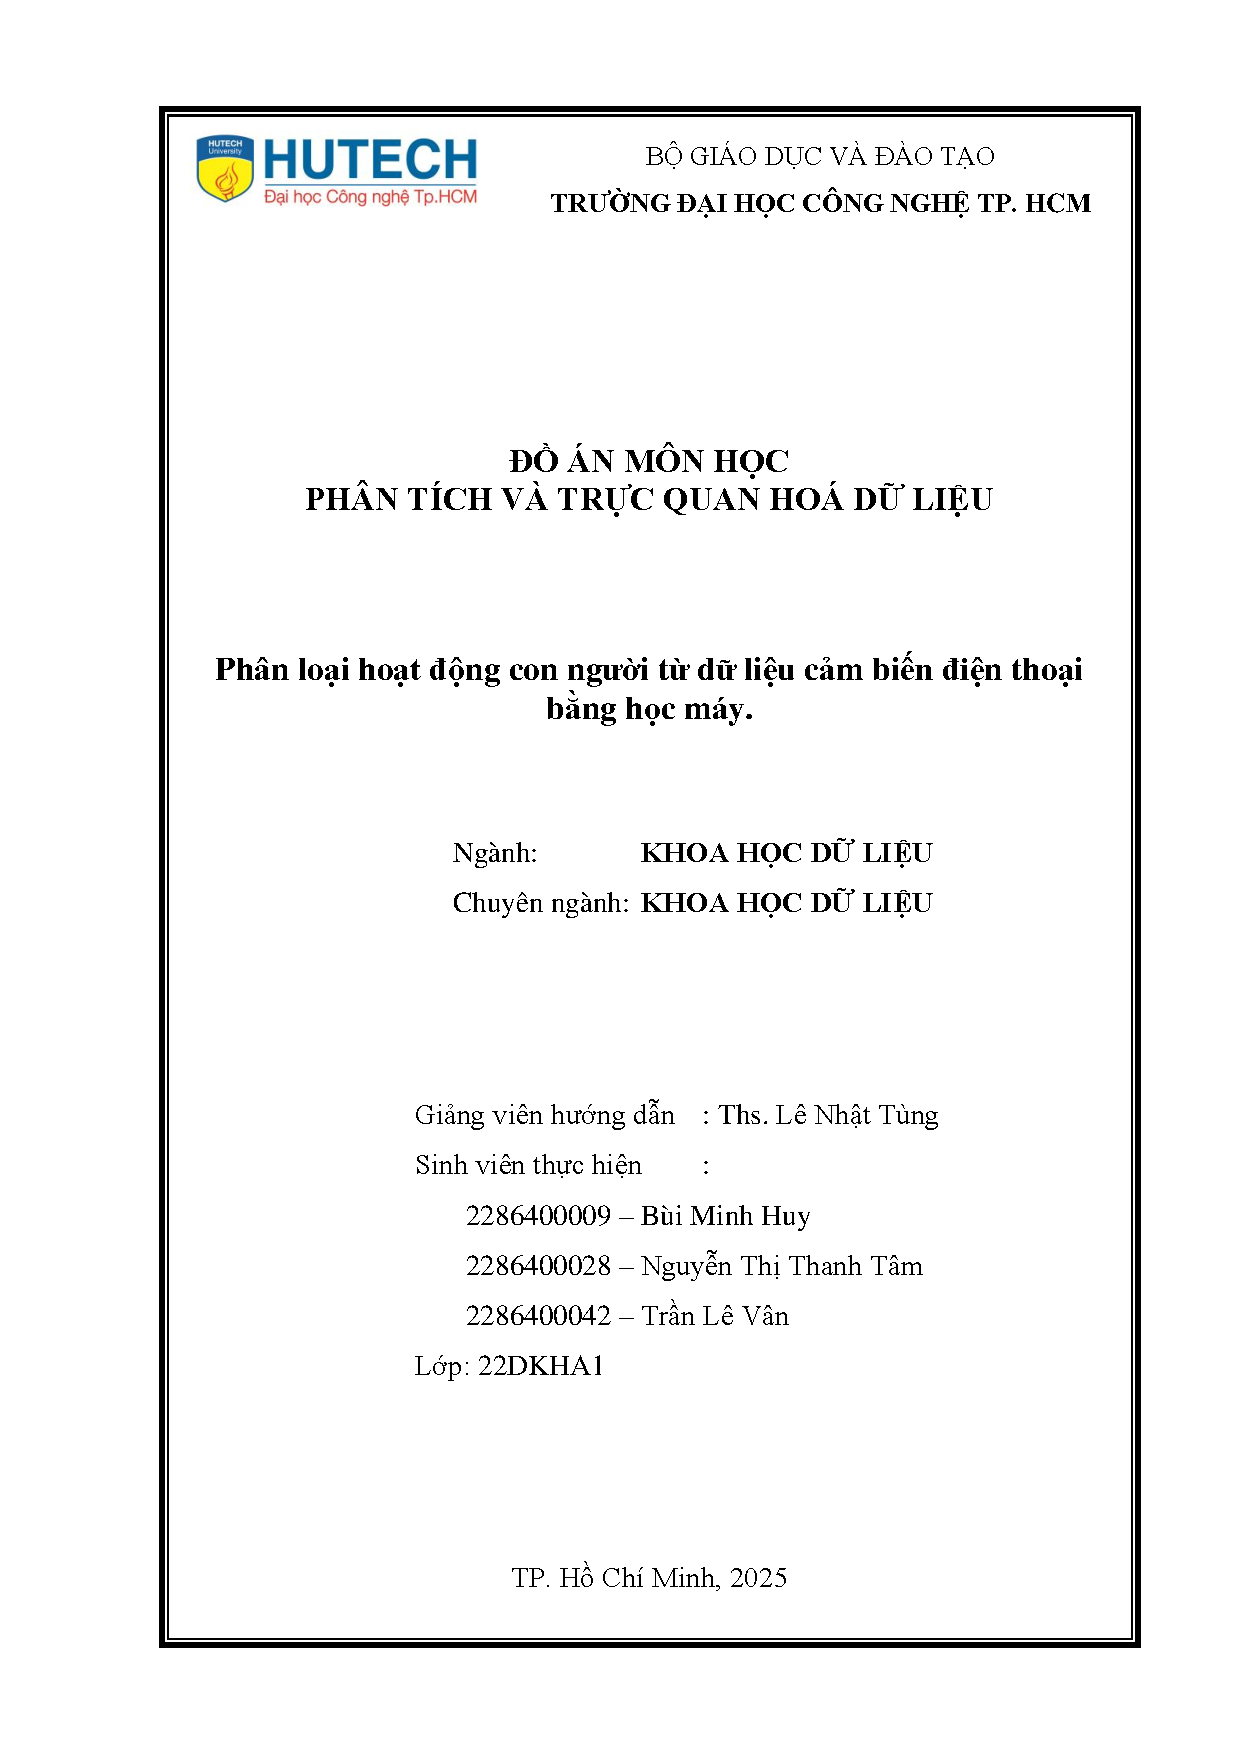
\includepdf[pages=1]{bia.pdf}
\pagenumbering{gobble}

\newpage
\thispagestyle{empty}

\begin{center}
    \LARGE {LỜI CAM ĐOAN}
\end{center}
\vspace{1.5em}

Chúng tôi, \textbf{Bùi Minh Huy}, \textbf{Trần Lê Vân}, \textbf{Nguyễn
Thị Thanh Tâm} xin cam đoan rằng:

Tất cả thông tin và phân tích trình bày trong báo cáo này được thực hiện
một cách chính xác và trung thực. Mọi dữ liệu, nhận định hoặc ý kiến
được trích dẫn từ các nguồn khác đều đã được nêu rõ nguồn gốc và trích
dẫn đúng quy định. Chúng tôi cam đoan rằng không có bất kỳ hành vi sao
chép hoặc sử dụng thông tin không hợp pháp nào từ các nguồn khác. Bài
báo cáo này là kết quả của công trình nghiên cứu độc lập của chúng tôi
và chưa từng được công bố tại bất kỳ nơi nào khác. Chúng tôi cam đoan đã
tuân thủ nghiêm ngặt các quy tắc và quy định của môn học, bao gồm việc
tham khảo và áp dụng các công cụ nghiên cứu một cách hợp lệ. Nếu phát
hiện có bất kỳ sự gian lận nào, chúng tôi xin hoàn toàn chịu trách nhiệm
về nội dung bài báo cáo của mình. Chúng tôi hy vọng rằng bài báo cáo này
sẽ cung cấp những thông tin hữu ích cho các nhà nghiên cứu, doanh
nghiệp, góp phần vào việc hiểu rõ hơn về mạng xã hội ngày nay.

\vspace{3em}

\begin{flushright}
\begin{minipage}{0.5\textwidth}
\raggedleft
TP.\ Hồ Chí Minh, ngày 28 tháng 3 năm 2025

\vspace{1em}

\centering
{\LARGE Sinh viên}
\end{minipage}
\end{flushright}

\newpage
\thispagestyle{empty}
\tableofcontents

\newpage
\thispagestyle{empty}
\listoffigures

\newpage
\pagenumbering{arabic}
\setcounter{page}{1}

\section*{CHƯƠNG 1: GIỚI THIỆU TỔNG QUAN}
\addcontentsline{toc}{section}{CHƯƠNG 1: GIỚI THIỆU TỔNG QUAN}
\setcounter{section}{1}

Trong thời đại của điện toán di động và thiết bị thông minh, việc theo
dõi và nhận dạng hoạt động con người (Human Activity Recognition - HAR)
đã trở thành một lĩnh vực nghiên cứu đóng vai trò quan trọng trong nhiều
ngành như trí tuệ nhân tạo, khoa học dữ liệu, y học và công nghệ cảm
biến. HAR đóng vai trò cốt lõi trong các ứng dụng như giám sát sức khỏe,
phát hiện té ngã, điều khiển nhà thông minh. Ngày nay, nhu cầu càng ngày
gia tăng về các thiết bị công nghệ có thể hiểu hành vi con người dẫn đến
việc phát triển các mô hình HAR là chính xác, hiệu quả và có khả năng
triển khai thực tế là vô cùng cần thết.

Một trong những yếu tố chính thúc đẩy sự phát triển của HAR là sự phổ
biến của các thiết bị di động thông minh và đồng hồ thông minh, vốn đợc
trang bị sẵn các cảm biến quán tính bao gồm gia tốc kế (accelerometer)
và con quay hồi chuyển (gyroscope). Những cảm biến này cho phép thu thập
dữ liệu về chuyển động của người sử dụng với độ chính xác cao, chi phí
thấp và tính khả dụng cao trong đời sống hàng ngày. Nhờ vậy, hệ thống
HAR có thể được lắp đặt mà không cần sử dụng các thiết bị đắt tiền hoặc
lắp đặt phức tạp.

Bên cạnh tiềm năng ứng dụng rộng rãi, việc xây dựng các mô hình HAR vẫn
có nhiều khó khăn thách thức như dữ liệu cảm biến thường có số chiều
lớn, có nhiều dữ liệu nhiễu và có tính biến động cao do phụ thuộc vào
thói quen và hình thể của mỗi người. Bên cạnh đó, một số hoạt động có
thể có mẫu tín hiệu tương tự nhau khiến cho các bài toán phân loại trở
nên khó khăn hơn. Vì vậy, cần có một quy trình xử lý dữ liệu bài bản bao
gồm các bước tiền xử lý dữ liệu, giảm chiều dữ liệu và huấn luyện mô
hình học máy để có thể đặt được hiệu quả cao trong việc nhận dạng hoạt
động con người.

Trong nghiên cứu này, chúng em đã tiến hành khai thác bộ dữ liệu
``\textbf{Human Activity Recognition with Smartphones}'' do UCI Machine
Learning Repository cung cấp, một bộ dữ liệu được sử dụng rộng rãi trong
cộng đồng nghiên cứu HAR. Chúng em đề xuất một quy trình học máy toàn
diện bao gồm phân tích đặc trưng, giảm chiều dữ liệu bằng UMAP, PCA,
TSNE và huấn luyện bằng các mô hình học máy như Random Forest, Decision
Tree, Logistic Regression, Support Vectot Machine (SVM) để phân loại các
hoạt động với mục tiêu là nâng cao độ chính xác và hiệu quả của mô hình.
Những kết quả này sẽ cung cấp cái nhìn thực nghiệm rõ ràng cho các nhà
nghiên cứu, đồng thời làm nền móng cho việc triển khai các hệ thống nhận
dạng hoạt động trong thế giới thực.

\section*{CHƯƠNG 2: CƠ SỞ LÝ THUYẾT}
\addcontentsline{toc}{section}{CHƯƠNG 2: CƠ SỞ LÝ THUYẾT}
\setcounter{section}{2}
\setcounter{subsection}{0}

\subsection{Hồi quy logistic (Logistic
Regression)}\label{hux1ed3i-quy-logistic-logistic-regression}

\subsubsection{Khái niệm}\label{khuxe1i-niux1ec7m}

Hồi quy logistic (Logistic Regression) là một thuật toán học máy có giám
sát (supervised learning), đồng thời cũng là một phương pháp thống kê
phổ biến, được sử dụng rộng rãi trong việc phân tích và dự đoán dữ liệu
phân loại. Mô hình này đặc biệt hiệu quả trong các bài toán phân loại
nhị phân, nơi mà biến phụ thuộc chỉ có hai giá trị khả dĩ như có/không,
đúng/sai hoặc 1/0.

Hồi quy logistic thường được ưu tiên sử dụng trong các bài toán dự đoán
khi biến phụ thuộc không phải là biến liên tục mà là biến nhị phân hoặc
phân loại, giúp cung cấp cái nhìn định lượng và chính xác về mối quan hệ
giữa các biến độc lập và xác suất xảy ra của sự kiện cần phân tích.

\subsubsection{Các loại hồi quy
logistic}\label{cuxe1c-loux1ea1i-hux1ed3i-quy-logistic}

\textbf{Hồi quy logistic nhị phân (Binary Logistic Regression)}. Hồi quy
logistic nhị phân dự đoán mối quan hệ giữa các biến phụ thuộc nhị phân
và độc lập . Một số ví dụ về đầu ra của loại hồi quy này có thể là thành
công/thất bại, 0/1 hoặc đúng/sai.

\textbf{Hồi quy logistic đa thức : (Multinomial Logistic Regression)}.
Biến phụ thuộc phân loại có hai hoặc nhiều kết quả rời rạc trong loại
hồi quy đa thức. Hồi quy logistic đa thức có nhiều hơn hai kết quả có
thể xảy ra .

\textbf{Hồi quy logistic thứ tự (Ordinal Logistic Regression)}. Hồi quy
logistic thứ tự áp dụng khi biến phụ thuộc ở trạng thái có thứ tự (tức
là thứ tự.

\subsubsection{Hàm Sigmoid}\label{huxe0m-sigmoid}

Hồi quy logistic dự đoán xác suất rơi vào một trong hai lớp (binary
classification), thường được ký hiệu là 0 hoặc 1.

Để biểu diễn xác suất này, sử dụng hàm sigmoid, có dạng S-shaped và giới
hạn giá trị đầu ra trong khoảng từ 0 đến 1.

Công thức của hàm sigmoid:

\[
S(z) = \frac{1}{1 + e^{-z}}
\]

Trong đó:

\begin{itemize}
\item
  s(z) = đầu ra trong khoảng từ 0 đến 1 (giá trị xác suất ước lượng).
\item
  z = đầu vào của hàm (giá trị dự đoán của thuật toán, ví dụ như mx+b).
\item
  e = hằng số Euler, và là cơ sở của logarithm tự nhiên.
\end{itemize}

\textbf{Đặc điểm mô hình:}

\begin{itemize}
\item
  Phân lớp và dự đoán: Dự đoán biến phụ thuộc nhị phân hoặc danh mục từ
  một hoặc nhiều biến độc lập.
\item
  Xác định mức độ ảnh hưởng của biến độc lập: Xác định cách thức và mức
  độ mà các biến độc lập ảnh hưởng đến xác suất của sự kiện hoặc lớp mục
  tiêu.
\item
  Tính toán xác suất sự kiện: Cung cấp ước lượng xác suất cho một sự
  kiện xảy ra dựa trên biến độc lập.
\end{itemize}

\subsubsection{Cách thức hoạt động của mô
hình}\label{cuxe1ch-thux1ee9c-houx1ea1t-ux111ux1ed9ng-cux1ee7a-muxf4-huxecnh}

Hồi quy logistic sử dụng hàm logistic (còn gọi là hàm sigmoid) để chuyển
đổi giá trị dự đoán thành xác suất. Hàm logistic có dạng:

Công thức của mô hình hồi quy logistic:

\[
P(Y = 1) = \frac{1}{1 + e^{-(\beta_0 + \beta_1 X_1 + \cdots + \beta_k X_k)}}
\]

Trong đó:

\emph{P(Y = 1)} là xác suất để sự kiện \emph{Y = 1} xảy ra (ví dụ: sự
kiện thành công, top 1,\ldots). \emph{X₁, X₂, \ldots, Xₖ} là các biến
độc lập. \emph{β₀, β₁, \ldots, βₖ} là hệ số mô hình cần được ước lượng.
\emph{e} là cơ số của logarithm tự nhiên.

\textbf{Cách hoạt động}

\begin{itemize}
\item
  \textbf{Ước lượng hệ số mô hình}: Hệ số β của mô hình được ước lượng
  thông qua quy trình tối ưu hóa, thường là phương pháp Maximum
  Likelihood Estimation (MLE).MLE tìm cách tối đa hóa xác suất của dữ
  liệu quan sát dựa trên hệ số β.
\item
  \textbf{Phân lớp}: Dựa vào xác suất được dự đoán từ hàm logistic,
  quyết định phân loại một quan sát vào lớp 1 nếu P(Y = 1) ≥ một ngưỡng
  cụ thể (thường là 0.5) và ngược lại là lớp 0. Ví dụ: Nếu P(Y = 1)
  \textgreater{} 0.5, quan sát được phân loại là lớp 1.
\item
  \textbf{Đánh giá mô hình:} Mô hình hồi quy logistic thường được đánh
  giá thông qua các chỉ số như độ chính xác (accuracy), precision,
  recall, điểm số F1, hoặc thống qua ROC và AUC.
\end{itemize}

\subsubsection{Nhược điểm của hồi quy
logistic}\label{nhux1b0ux1ee3c-ux111iux1ec3m-cux1ee7a-hux1ed3i-quy-logistic}

\begin{itemize}
\tightlist
\item
  Không thích hợp với biến phụ thuộc liên tục.
\item
  khó khăn trong việc mô hình hóa mối quan hệ phức tạp hoặc không tuyến
  tính mà không cần biến đổi dữ liệu.
\item
  Không hiệu quả khi xử lý dữ liệu có nhiều biến độc lập hoặc có sự
  tương quan cao giữa các biến.
\end{itemize}

\subsection{K-Nearest Neighbors (KNN)}\label{k-nearest-neighbors-knn}

\subsubsection{Khái niệm}\label{khuxe1i-niux1ec7m-1}

K-Nearest Neighbors (KNN) là một trong những thuật toán học máy đơn giản
nhất nhưng hiệu quả, thuộc nhóm học có giám sát (supervised learning).
Thuật toán được sử dụng cho cả hai bài toán phân lớp (classification) và
hồi quy (regression), tuy nhiên nó phổ biến hơn trong các bài toán phân
lớp. Ý tưởng của thuật toán này là nó không học một điều gì từ tập dữ
liệu học (nên KNN được xếp vào loại lazy learning), mọi tính toán được
thực hiện khi nó cần dự đoán nhãn của dữ liệu mới.

\subsubsection{Cách thức hoạt động của thuật toán
KNN}\label{cuxe1ch-thux1ee9c-houx1ea1t-ux111ux1ed9ng-cux1ee7a-thuux1eadt-touxe1n-knn}

Bước 1: Chọn một số nguyên K (số lượng hàng xóm gần nhất cần xét).

Bước 2: Tính khoảng cách của data input với các data trong có trong tập
data train, có các cách tính khoảng cách như: Minkowski, Euclid,
Manhattan, \ldots{} tùy mục đích sử dụng mà chúng ta sử dụng cách tính
khoảng cách, thông dụng nhất là cách tính Euclid.

Bước 3: Sau khi tính khoảng cách từ data input tới toàn bộ data trong
tập training, chọn ra K lân cận với khoảng cách ngắn nhất, với K được
chọn ở bước số 1.

Bước 4: Thực hiện phân loại, kết quả sẽ theo label có tỉ lệ voting cao
nhất.

\textbf{Lựa chọn giá trị K}

\begin{itemize}
\tightlist
\item
  Giá trị K quá nhỏ (ví dụ K = 1): mô hình nhạy cảm với nhiễu (noise),
  dễ bị overfitting.
\item
  Giá trị K quá lớn: mô hình quá ``mềm'', dễ bị underfitting
\end{itemize}

\subsubsection{Ưu điểm}\label{ux1b0u-ux111iux1ec3m}

\begin{itemize}
\tightlist
\item
  Đơn giản, dễ hiểu: Thuật toán có nguyên lý hoạt động trực quan, dễ cài
  đặt.
\item
  Không cần huấn luyện: Không tốn thời gian xây dựng mô hình.
\item
  Hiệu quả với dữ liệu nhỏ: Hoạt động tốt với tập dữ liệu kích thước vừa
  phải.
\item
  Ứng dụng đa dạng: Có thể áp dụng cho cả bài toán phân lớp và hồi quy.
\item
  Không có giả định về dữ liệu: Là mô hình phi tham số, không yêu cầu dữ
  liệu tuân theo phân phối cụ thể.
\item
  Thích ứng tốt với dữ liệu mới: Dễ dàng cập nhật mô hình bằng cách thêm
  mẫu mới.
\end{itemize}

\subsubsection{Nhược điểm}\label{nhux1b0ux1ee3c-ux111iux1ec3m}

\begin{itemize}
\tightlist
\item
  Chi phí dự đoán cao: Phải tính khoảng cách đến mọi mẫu dữ liệu, tốn
  kém với dữ liệu lớn.
\item
  Nhạy cảm với quy mô dữ liệu: Các đặc trưng có phạm vi lớn sẽ áp đảo
  các đặc trưng có phạm vi nhỏ.
\item
  Nhạy cảm với nhiễu và dữ liệu thừa: Kém hiệu quả khi có nhiều đặc
  trưng không liên quan.
\item
  Vấn đề với dữ liệu không cân bằng: Các lớp thịnh hành có xu hướng áp
  đảo các lớp thiểu số.
\item
  Khó chọn k tối ưu: Giá trị k thích hợp phụ thuộc vào dữ liệu cụ thể.
\end{itemize}

\subsection{Support Vector Machine
(SVM)}\label{support-vector-machine-svm}

\subsubsection{Khái niệm}\label{khuxe1i-niux1ec7m-2}

SVM là một thuật toán học máy có giám sát (supervised learning), dùng để
giải quyết các bài toán phân loại và hồi quy.

Mục tiêu chính của SVM là tìm một siêu phẳng (hyperplane) tốt nhất để
phân tách các điểm dữ liệu thuộc hai lớp khác nhau sao cho khoảng cách
(margin) giữa siêu phẳng và các điểm gần nhất của mỗi lớp là lớn nhất.

Điểm dữ liệu gần nhất đó được gọi là vector hỗ trợ (support vector). SVM
sử dụng các hàm kernel để biểu diễn không gian dữ liệu ban đầu vào không
gian cao chiều hơn, giúp phân loại tốt hơn đối với các bài toán phức
tạp.

\subsubsection{Các loại SVM}\label{cuxe1c-loux1ea1i-svm}

Trong thuật toán SVM, có hai loại chính là Linear SVM (SVM tuyến tính)
và Non-linear SVM (SVM phi tuyến).

Linear SVM là loại SVM mà ta có thể phân chia dữ liệu bằng một đường
thẳng. Điều này áp dụng cho các bài toán có dữ liệu tuyến tính và có thể
tách biệt bằng một đường thẳng.

Non-linear SVM được sử dụng khi không thể phân chia dữ liệu bằng một
đường thẳng. Trong trường hợp này, ta sẽ sử dụng các phương pháp biến
đổi dữ liệu sao cho chúng trở thành tuyến tính, sau đó áp dụng Linear
SVM để giải quyết bài toán.

\subsubsection{Cách hoạt động}\label{cuxe1ch-houx1ea1t-ux111ux1ed9ng}

\begin{itemize}
\tightlist
\item
  Chọn siêu phẳng phân tách: SVM tìm kiếm siêu phẳng sao cho có khoảng
  cách margin lớn nhất giữa hai lớp dữ liệu.
\item
  Tối đa hóa margin: Cố gắng duy trì khoảng cách lớn nhất từ siêu phẳng
  tới các điểm dữ liệu gần nhất.
\item
  Áp dụng kernel nếu cần: Nếu dữ liệu không phân tách tuyến tính, áp
  dụng kernel trick để biến đổi không gian dữ liệu.
\item
  Đánh giá và điều chỉnh tham số để tối ưu mô hình.
\end{itemize}

\subsubsection{Margin trong SVM}\label{margin-trong-svm}

Margin là khoảng cách từ siêu phẳng phân tách (hyperplane) đến các điểm
dữ liệu gần nhất thuộc hai lớp khác nhau -- các điểm này được gọi là
vector hỗ trợ (support vectors). Trong hình dung đơn giản, ví dụ như bài
toán phân loại quả táo và quả lê đặt trên mặt bàn, margin chính là
khoảng cách từ cây que (đại diện cho siêu phẳng) đến quả táo và quả lê
gần cây que nhất. Điều quan trọng trong SVM là thuật toán luôn tìm cách
tối đa hóa margin này, nhằm tạo ra một siêu phẳng phân tách có khoảng
cách lớn nhất đến các điểm dữ liệu gần ranh giới nhất của mỗi lớp. Nhờ
đó, SVM có thể tăng cường khả năng tổng quát hóa và giảm thiểu nguy cơ
phân loại sai khi xử lý các điểm dữ liệu mới chưa từng thấy trước đó.

\subsubsection{Thủ thuật Kernel}\label{thux1ee7-thuux1eadt-kernel}

Kernel là một hàm ánh xạ dữ liệu từ không gian ít nhiều hơn sang không
gian nhiều chiều hơn, từ đó ta tìm được siêu phẳng phân tách dữ liệu.
Một cách trực quan, kỹ thuật này giống như việc bạn gập tờ giấy lại để
có thể dùng kéo cắt một lỗ tròn trên nó.

\subsubsection{Ưu điểm}\label{ux1b0u-ux111iux1ec3m-1}

\begin{itemize}
\tightlist
\item
  Xử lý trên không gian số chiều cao: SVM là một công cụ tính toán hiệu
  quả trong không gian chiều cao, trong đó đặc biệt áp dụng cho các bài
  toán phân loại văn bản và phân tích quan điểm nơi chiều có thể cực kỳ
  lớn.
\item
  Tiết kiệm bộ nhớ: Do chỉ có một tập hợp con của các điểm được sử dụng
  trong quá trình huấn luyện và ra quyết định thực tế cho các điểm dữ
  liệu mới.
\item
  Tính linh hoạt - phân lớp thường là phi tuyến tính. Khả năng áp dụng
  Kernel mới phép linh động giữa các phương pháp tuyến tính và phi tuyến
  tính từ đó khiếncho hiệu suất phân loại lớn hơn.
\end{itemize}

\subsubsection{Nhược điểm}\label{nhux1b0ux1ee3c-ux111iux1ec3m-1}

\begin{itemize}
\tightlist
\item
  Thuật toán SVM có độ phức tạp tính toán cao khi số lượng dữ liệu lớn.
\item
  SVM yêu cầu dữ liệu huấn luyện là tuyến tính hoặc phi tuyến tính.
\item
  Thuật toán SVM cần lựa chọn tham số tốt để đạt được kết quả tốt nhất.
\end{itemize}

\subsection{Decision Tree}\label{decision-tree}

\subsubsection{Khái niệm}\label{khuxe1i-niux1ec7m-3}

Cây quyết định (Decision Tree) là một trong những thuật toán phổ biến
nhất trong lĩnh vực máy học (Machine Learning). Là một công cụ mạnh mẽ,
thường được sử dụng để giải quyết các bài toán về phân loại
(classification) và dự đoán (regression) trong khai phá dữ liệu. Cây
quyết định là một thuật toán máy học dùng để dự đoán hoặc phân loại dữ
liệu dựa trên các bước ra quyết định nối tiếp nhau.

\subsubsection{Cách hoạt động}\label{cuxe1ch-houx1ea1t-ux111ux1ed9ng-1}

Cách hoạt động của cây quyết định rất đơn giản:

\begin{itemize}
\item
  Đầu tiên, cây quyết định sẽ xem xét toàn bộ tập dữ liệu.
\item
  Sau đó, chia dữ liệu thành các nhóm nhỏ dựa trên một số đặc điểm hoặc
  điều kiện nhất định (ví dụ như tuổi tác, thu nhập, màu sắc, nhiệt
  độ..).
\item
  Việc chia nhỏ này sẽ tiếp tục thực hiện đến khi dữ liệu ở mỗi nhóm trở
  nên rõ ràng và dễ dàng để dự đoán hoặc phân loại.

  Trong cây quyết định, mỗi ``nút'' (node) đại diện cho một đặc điểm (ví
  dụ: ``tuổi'', ``mức thu nhập'', ``thời tiết''). Các ``nhánh'' (branch)
  nối giữa các nút chính là các điều kiện để chia dữ liệu (ví dụ: tuổi
  lớn hơn hay nhỏ hơn 30). Cuối cùng, các ``nút lá'' (leaf node) là kết
  quả cuối cùng mà cây quyết định đưa ra, ví dụ như ``mua hàng'' hay
  ``không mua hàng'', ``đi chơi thể thao'' hay ``ở nhà''.

  Nói cách khác, cây quyết định giống như một chuỗi các câu hỏi đơn giản
  được sắp xếp theo từng bước, giúp ta dễ dàng đi đến một quyết định
  cuối cùng.
\end{itemize}

\subsubsection{Công thức}\label{cuxf4ng-thux1ee9c}

\textbf{Gini Impurity}

Công thức Gini Impurity được sử dụng trong thuật toán cây quyết định để
đo lường độ không chính xác của một dự đoán khi phân loại một tập dữ
liệu.

Cần lưu ý là Gini Impurity càng nhỏ (gần 0) thì tập dữ liệu đó càng
``thuần khiết'', nghĩa là các mẫu trong cùng một nhóm có xu hướng thuộc
vào cùng một lớp. Ngược lại, nếu Gini Impurity cao (gần 1), thì việc
phân loại các mẫu trong nhóm đó trở nên không chắc chắn.

Giả sử khi đang xem xét một tập dữ liệu chia thành K nhóm, mỗi nhóm chứa
một phần tỷ lệ pi với i=1,2,\ldots,K.

Công thức tính độ bất thuần Gini (Gini Impurity):

\[
I_G = 1 - \sum_{i=1}^{K} p_i^2
\]

Trong đó:

\begin{itemize}
\item
  \emph{\(I_G\)} là Gini Impurity.
\item
  \emph{\(p_i\)} là tỷ lệ các mẫu thuộc vào lớp \emph{\(i\)}.

  Khi xây dựng cây quyết định, chúng ta cần chọn thuộc tính và giá trị
  phân chia sao cho Gini Impurity sau phân chia là nhỏ nhất, tức là mức
  độ ``thuần khiết'' cho dữ liệu thuộc về từng nhóm con được tạo ra.
\end{itemize}

\textbf{Entropy}

Entropy trong cây quyết định là một khái niệm được sử dụng để đo lường
sự không chắc chắn trong dữ liệu (Trung bình surprise). Trong ngữ cảnh
của cây quyết định, entropy thường được sử dụng để đo lường mức độ không
chắc chắn của phân phối lớp trong tập dữ liệu.

Entropy được tính bằng công thức sau: \[
\text{Entropy}(S) = - \sum_{i=1}^{c} p_i \log_2(p_i)
\]

Trong đó:

\begin{itemize}
\item
  \emph{\(S\)} là tập dữ liệu.
\item
  \emph{\(c\)} là số lớp trong tập dữ liệu.
\item
  \emph{\(p_i\)} là tỷ lệ của lớp \emph{\(i\)} trong tập dữ liệu.

  Entropy càng cao khi tỷ lệ của các lớp trong tập dữ liệu gần bằng
  nhau, và càng thấp khi một lớp chiếm đa số.

  Khi xây dựng cây quyết định, chúng ta cố gắng chia tập dữ liệu sao cho
  entropy sau khi chia là thấp nhất có thể. Điều này giúp cây quyết định
  có thể học được các quy tắc quyết định hiệu quả từ dữ liệu.

  Quyết định về cách chia tập dữ liệu dựa trên entropy thường được thực
  hiện bằng cách so sánh entropy trước và sau khi chia, và chọn cách
  chia mà giảm entropy nhiều nhất.
\end{itemize}

\subsubsection{Ưu điểm}\label{ux1b0u-ux111iux1ec3m-2}

\begin{itemize}
\tightlist
\item
  Mô hình sinh ra các quy tắc dễ hiểu cho người đọc, tạo ra bộ luật với
  mỗi nhánh lá là một luật của cây.
\item
  Dữ liệu đầu vào có thể là dữ liệu missing, không cần chuẩn hóa hoặc
  tạo biến giả.
\item
  Có thể làm việc với cả dữ liệu số và dữ liệu phân loại.
\item
  Có thể xác thực mô hình bằng cách sử dụng các kiểm tra thống kê.
\item
  Có khả năng làm với dữ liệu lớn.
\end{itemize}

\subsubsection{Nhược điểm}\label{nhux1b0ux1ee3c-ux111iux1ec3m-2}

\begin{itemize}
\tightlist
\item
  Mô hình cây quyết định phụ thuộc rất lớn vào dữ liệu. Thậm chí, với
  một sự thay đổi nhỏ trong bộ dữ liệu, cấu trúc mô hình cây quyết định
  có thể thay đổi hoàn toàn.
\item
  Cây quyết định hay gặp vấn đề overfitting
\end{itemize}

\subsubsection{Các vấn đề sau khi thực hiện áp dụng mô hình vào dữ liệu
cần dự
đoán}\label{cuxe1c-vux1ea5n-ux111ux1ec1-sau-khi-thux1ef1c-hiux1ec7n-uxe1p-dux1ee5ng-muxf4-huxecnh-vuxe0o-dux1eef-liux1ec7u-cux1ea7n-dux1ef1-ux111ouxe1n}

\textbf{Underfitting:}là hiện tượng kết quả độ chênh lệch của mô hình
được huấn luyện và kết quả độ chênh lệch của dữ liệu cần dự đoán đạt giá
trị mức cao giống nhau, do mô hình chưa được huấn luyện đầy đủ. Cần xem
lại cấu trúc của mô hình (tăng thêm độ phức tạp) để có thể huấn luyện
các tập dữ liệu khó và tăng thêm dữ liệu huấn luyện để tăng hiệu suất
của mô hình.

\textbf{Overfitting:}là hiện tượng kết quả của mô hình được huấn luyện
quá tốt (độ chênh lệch thấp) nhưng khi áp dụng vào dữ liệu cần dự đoán
thì mô hình đạt hiêu suất kém (độ chênh lệch cao) do mô hình đã học quát
sát với dữ liệu huấn luyện và không có khả năng tổng quát hóa các dữ
liệu cần dự đoán. Cần sử dụng một số các phương pháp tránh overfitting
như tăng độ đa dạng của dữ liệu, giảm thiểu độ phức tạp của mô hình.

=\textgreater{} Giải pháp : Pruning solution là được áp dụng đối với
trường hợp mô hình huấn uyện bị overfitting khi sử dụng mô hình Decision
Tree bằng cách hạn chế kích thước, chiều sâu của mô hình này.

\subsection{Random Forest}\label{random-forest}

\subsubsection{Khái niệm}\label{khuxe1i-niux1ec7m-4}

Random Forest là một thuật toán học máy thuộc nhóm học có giám sát
(supervised learning), được sử dụng phổ biến trong cả bài toán phân loại
và hồi quy.

Khác với Decision Tree chỉ dựa vào một cây duy nhất, Random Forest kết
hợp nhiều cây quyết định để tạo ra một mô hình tổng hợp, có khả năng dự
đoán chính xác và ổn định hơn.

\subsubsection{Cách hoạt động của Random
Forest}\label{cuxe1ch-houx1ea1t-ux111ux1ed9ng-cux1ee7a-random-forest}

\begin{itemize}
\tightlist
\item
  Tạo ra nhiều cây khác nhau từ các tập dữ liệu nhỏ, được chọn ngẫu
  nhiên từ tập dữ liệu gốc.
\item
  Mỗi cây sẽ đưa ra dự đoán riêng.
\item
  Mô hình sẽ lấy trung bình (với hồi quy) hoặc bỏ phiếu theo số đông
  (với phân loại) để đưa ra kết quả cuối cùng.
\end{itemize}

\subsubsection{Công thức}\label{cuxf4ng-thux1ee9c-1}

Bài toán phân loại (classification) Bài toán phân loại, mỗi cây quyết
định trong rừng sẽ đưa ra một nhãn dự đoán. Sau đó, mô hình Random
Forest sẽ lấy nhãn xuất hiện nhiều nhất trong các dự đoán của từng cây
làm kết quả cuối cùng.

Công thức được biểu diễn như sau:

\[
\hat{y} = \text{mode}(h_1(x), h_2(x), \ldots, h_T(x))
\]

Trong đó:

\begin{itemize}
\item
  \emph{\(\hat{y}\)} là kết quả dự đoán cuối cùng của mô hình.
\item
  \emph{\(h_t(x)\)} là kết quả dự đoán của cây thứ \emph{\(t\)} với đầu
  vào \emph{\(x\)}.
\item
  \emph{\(T\)} là tổng số cây trong mô hình Random Forest.
\item
  \emph{mode} là hàm chọn giá trị xuất hiện nhiều nhất.

  Bài toán hồi quy (Regression Với bài toán hồi quy, mỗi cây trong rừng
  sẽ đưa ra một giá trị số. Kết quả cuối cùng được tính bằng cách lấy
  trung bình cộng các giá trị dự đoán của tất cả các cây.
\end{itemize}

Được tính bằng công thức sau:

\[
\hat{y} = \frac{1}{T} \sum_{t=1}^{T} h_t(x)
\]

Trong đó:

\begin{itemize}
\tightlist
\item
  \emph{\(\hat{y}\)} là giá trị dự đoán cuối cùng.
\item
  \emph{\(h_t(x)\)} là giá trị dự đoán từ cây thứ \emph{\(t\)}.
\item
  \emph{\(T\)} là tổng số cây trong mô hình.
\end{itemize}

\subsubsection{Ưu điểm}\label{ux1b0u-ux111iux1ec3m-3}

\begin{itemize}
\item
  Độ chính xác cao: mô hình tổng hợp nhiều cây, Random Forest thường cho
  kết quả chính xác hơn so với cây quyết định đơn lẻ.
\item
  Chống overfitting tốt: kết hợp nhiều cây được huấn luyện từ dữ liệu và
  thuộc tính ngẫu nhiên giúp mô hình tránh học quá sát vào dữ liệu huấn
  luyện.
\item
  Làm việc tốt với dữ liệu lớn và có nhiều đặc trưng: Random Forest xử
  lý hiệu quả dữ liệu có số chiều lớn và phức tạp.
\item
  Không yêu cầu chuẩn hóa dữ liệu: Dữ liệu đầu vào không cần phải được
  chuẩn hóa hoặc xử lý đặc biệt như một số thuật toán khác.
\item
  Có thể đo lường mức độ quan trọng của các thuộc tính (feature
  importance): Giúp phân tích và chọn ra các yếu tố ảnh hưởng nhiều nhất
  đến kết quả dự đoán.
\end{itemize}

\subsubsection{Nhược điểm}\label{nhux1b0ux1ee3c-ux111iux1ec3m-3}

\begin{itemize}
\item
  Khó giải thích mô hình: Random Forest gồm nhiều cây nên khó để xem
  toàn bộ quátrình mô hình đưa ra kết quả , khó để giải thích được mô
  hình .
\item
  Thời gian huấn luyện và dự đoán lâu hơn: Mô hình gồm nhiều cây nên tốn
  nhiều thời gian và tài nguyên hơn khi xử lý dữ liệu lớn.
\item
  Chiếm nhiều bộ nhớ: Lưu trữ nhiều cây có thể tốn nhiều RAM, đặc biệt
  khi số lượng cây lớn.
\item
  Dễ bị bias nếu dữ liệu không cân bằng: Trong trường hợp dữ liệu bị
  lệch, Random Forest có thể dự đoán thiên lệch theo lớp đó nếu không xử
  lý cân bằng dữ liệu trước.
\end{itemize}

\subsection{UMAP}\label{umap}

\subsubsection{Khái niệm}\label{khuxe1i-niux1ec7m-5}

\textbf{Uniform Manifold Approximation and Projection (UMAP)} là một kỹ
thuật giảm chiều dữ liệu, tương tự như t-SNE, thường được sử dụng để
trực quan hóa dữ liệu. Ngoài ra, UMAP còn có thể được sử dụng như một
phương pháp giảm chiều phi tuyến tổng quát trong các bài toán học máy.
Thuật toán UMAP được xây dựng dựa trên ba giả định chính về cấu trúc dữ
liệu: 1. Dữ liệu phân bố đều trên một đa tạp Riemannian (Riemannian
manifold); 2. Metric Riemannian là hằng số cục bộ (hoặc có thể được xấp
xỉ là như vậy); 3. Ống phân phối (local connectivity) được kết nối cục
bộ.

\subsubsection{Mục tiêu của UMAP}\label{mux1ee5c-tiuxeau-cux1ee7a-umap}

• Giảm số lượng biến: UMAP chuyển đổi dữ liệu sang một không gian có số
chiều thấp hơn, phù hợp cho các tác vụ xử lý và phân tích tiếp theo.

\begin{itemize}
\item
  Giữ lại cấu trúc dữ liệu: UMAP cố gắng bảo toàn cả cấu trúc cục bộ
  (local structure) lẫn cấu trúc tổng thể (global structure) của dữ liệu
  trong không gian mới.
\item
  Bảo tồn mối quan hệ phi tuyến: Khác với PCA, UMAP có khả năng nắm bắt
  và biểu diễn các mối quan hệ phi tuyến giữa các điểm dữ liệu.
\item
  Trực quan hóa dữ liệu: UMAP đặc biệt hiệu quả trong việc trực quan hóa
  dữ liệu nhiều chiều trong không gian 2D hoặc 3D, với độ chính xác và
  sắc nét cao hơn so với nhiều kỹ thuật khác như t-SNE.
\end{itemize}

\subsubsection{Quy trình thực hiện
UMAP}\label{quy-truxecnh-thux1ef1c-hiux1ec7n-umap}

\begin{itemize}
\tightlist
\item
  Chuẩn hóa dữ liệu (nếu cần).
\item
  Tìm k hàng xóm gần nhất cho mỗi điểm và xây dựng đồ thị fuzzy biểu
  diễn cấu trúc cục bộ.
\item
  Tính toán xác suất kết nối giữa các điểm dựa trên khoảng cách và hàm
  kernel.
\item
  Khởi tạo các điểm trong không gian thấp chiều và tối ưu hóa đồ thị sao
  cho bảo toàn cấu trúc so với đồ thị ban đầu.
\item
  Chiếu dữ liệu sang không gian mới để phục vụ trực quan hóa hoặc các
  bước phân tích tiếp theo.
\end{itemize}

\subsubsection{Ưu điểm}\label{ux1b0u-ux111iux1ec3m-4}

\begin{itemize}
\tightlist
\item
  Bảo toàn cấu trúc cục bộ tốt.
\item
  Có thể dùng cho cả supervised \& unsupervised.
\item
  UMAP cho phép lưu và áp dụng mô hình lên dữ liệu mới.
\end{itemize}

\subsubsection{Nhược điểm}\label{nhux1b0ux1ee3c-ux111iux1ec3m-4}

\begin{itemize}
\tightlist
\item
  Không giải thích được biến gốc.
\item
  Phụ thuộc vào tham số.
\end{itemize}

\section*{CHƯƠNG 3: GIỚI THIỆU BỘ DỮ LIỆU}
\addcontentsline{toc}{section}{CHƯƠNG 3: GIỚI THIỆU BỘ DỮ LIỆU}
\setcounter{section}{3}

Bộ dữ liệu \textbf{Human Activity Recognition with Smartphones} được xây
dựng nhằm phục vụ cho các nghiên cứu về nhận diện hành vi con người
thông qua dữ liệu cảm biến thu thập từ thiết bị di động. Tập dữ liệu
được thu thập từ 30 người tham gia (gọi là \emph{subjects}) (15 nam và
15 nữ, độ tuổi từ 19 đến 48) thực hiện sáu hoạt động thường ngày như Đi
bộ (Walking), đi lên cầu thang (Walking Upstairs), đi xuống cầu thang
(WalkingDownstairs), ngồi (Sitting), đứng (Standing)và nằm (Laying).

Dữ liệu được ghi lại bằng một điện thoại thông minh (Samsung Galaxy S
II) đeo ở thắt lưng của người dùng. Thiết bị này sử dụng hai loại cảm
biến là \textbf{accelerometer} và \textbf{gyroscope} được sử dụng để ghi
lại chuyển động theo 3 trục X, Y, Z với tần số lấy mẫu 50Hz.

Mỗi chuỗi tín hiệu được chia thành các \textbf{cửa sổ trượt} có độ dài
2.56 giây, tương ứng với 128 lần đo. Từ mỗi cửa sổ, các đặc trưng
(features) đã được trích xuất từ \textbf{miền thời gian} và \textbf{miền
tần số} để tạo ra một tập hợp dữ liệu có cấu trúc sẵn sàng cho mô hình
học máy.

Các tín hiệu chính được sử dụng để tạo đặc trưng bao gồm:

\begin{itemize}
\tightlist
\item
  \texttt{tBodyAcc-XYZ}: Gia tốc cơ thể theo 3 trục trong miền thời
  gian\\
\item
  \texttt{tGravityAcc-XYZ}: Gia tốc do trọng lực\\
\item
  \texttt{tBodyGyro-XYZ}: Tốc độ quay từ con quay hồi chuyển\\
\item
  \texttt{tBodyAccJerk-XYZ}, \texttt{tBodyGyroJerk-XYZ}: Jerk - đo sự
  thay đổi đột ngột của chuyển động\\
\item
  \texttt{Mag}: Độ lớn vector gia tốc, được tính bằng chuẩn Euclidean:\\
  \[
  \text{Mag} = \sqrt{X^2 + Y^2 + Z^2}
  \]
\item
  \texttt{fBodyAcc-XYZ}, \texttt{fBodyGyro-XYZ}: Biến miền tần số được
  tạo từ FFT
\end{itemize}

Từ các tín hiệu trên, 561 đặc trưng thống kê đã được trích xuất, bao
gồm:

\begin{itemize}
\item
  \texttt{mean()}, \texttt{std()}, \texttt{mad()}, \texttt{max()},
  \texttt{min()}: Đặc trưng thông kê truyền thống
\item
  \texttt{sma()}: Signal Magnitude Area
\item
  \texttt{energy()}: Tổng bình phương chia số phần tử
\item
  \texttt{entropy()}, \texttt{iqr()}, \texttt{arCoeff()},
  \texttt{correlation()}
\item
  \texttt{meanFreq()}, \texttt{skewness()}, \texttt{kurtosis()},
  \texttt{bandsEnergy()}, \texttt{angle()}

  Toàn bộ bộ dữ liệu được chia thành hai phần: Tập huấn luyện
  (train.csv): bao gồm 7352 mẫu. Tập kiểm tra (test.csv): bao gồm 2947
  mẫu. Mỗi mẫu tương ứng với một cửa sổ thời gian 2.56 giây, được biểu
  diễn bằng \textbf{561 đặc trưng đầu vào (features)}, cùng với một mã
  định danh người thực hiện (subject) và một nhãn hoạt động (Activity),
  các nhãn này được mã hóa từ 1 đến 6 tương ứng với:
\end{itemize}

\begin{longtable}[]{@{}ll@{}}
\toprule\noalign{}
Giá trị nhãn & Hoạt động \\
\midrule\noalign{}
\endhead
\bottomrule\noalign{}
\endlastfoot
1 & WALKING \\
2 & WALKING\_UPSTAIRS \\
3 & WALKING\_DOWNSTAIRS \\
4 & SITTING \\
5 & STANDING \\
6 & LAYING \\
\end{longtable}

\begin{Shaded}
\begin{Highlighting}[]
\CommentTok{\# install.packages("showtext")}
\CommentTok{\# install.packages("ggplot2")}
\end{Highlighting}
\end{Shaded}

\begin{Shaded}
\begin{Highlighting}[]
\CommentTok{\# train \textless{}{-}read.csv(\textquotesingle{}/Users/huy/Documents/doanthaytung/archive/train.csv\textquotesingle{})}
\CommentTok{\# train \textless{}{-}read.csv("D:/BT/clonegit/doanthaytung/archive/train.csv")}
\NormalTok{train }\OtherTok{\textless{}{-}} \FunctionTok{read.csv}\NormalTok{(}\StringTok{\textquotesingle{}archive/train.csv\textquotesingle{}}\NormalTok{)}
\CommentTok{\# head(train)}
\FunctionTok{dim}\NormalTok{(train)}
\end{Highlighting}
\end{Shaded}

\begin{verbatim}
## [1] 7352  563
\end{verbatim}

\begin{Shaded}
\begin{Highlighting}[]
\CommentTok{\# test \textless{}{-}read.csv(\textquotesingle{}/Users/huy/Documents/doanthaytung/archive/test.csv\textquotesingle{})}
\CommentTok{\# test \textless{}{-}read.csv("D:/BT/clonegit/doanthaytung/archive/test.csv")}
\NormalTok{test }\OtherTok{\textless{}{-}} \FunctionTok{read.csv}\NormalTok{(}\StringTok{"archive/test.csv"}\NormalTok{)}
\CommentTok{\# head(test)}
\FunctionTok{dim}\NormalTok{(test)}
\end{Highlighting}
\end{Shaded}

\begin{verbatim}
## [1] 2947  563
\end{verbatim}

\begin{itemize}
\tightlist
\item
  Kiểm tra kiểu dữ liệu của các biến trong tập huấn luyện để thống kê số
  lượng cột thuộc từng kiểu dữ liệu trong bảng dữ liệu train. Kết quả sẽ
  cung cấp một cái nhìn tổng quan về cấu trúc dữ liệu, giúp đánh giá mức
  độ sẵn sàng của tập dữ liệu cho các bước xử lý tiếp theo.
\end{itemize}

\begin{Shaded}
\begin{Highlighting}[]
\FunctionTok{table}\NormalTok{(}\FunctionTok{sapply}\NormalTok{(train, class))}
\end{Highlighting}
\end{Shaded}

\begin{verbatim}
## 
## character   integer   numeric 
##         1         1       561
\end{verbatim}

Theo kết quả trả về, bộ dữ liệu train bao gồm: 561 biến kiểu numeric, 1
biến kiểu character, 1 biến kiểu integer.

\begin{itemize}
\tightlist
\item
  Kiểm tra xem có biến nào được lưu dưới dạng chuỗi ký tự (character)
  hay không. Đảm bảo các biến phân loại sẽ được xử lý đúng cách trong mô
  hình học máy.
\end{itemize}

\begin{Shaded}
\begin{Highlighting}[]
\FunctionTok{names}\NormalTok{(train)[}\FunctionTok{sapply}\NormalTok{(train, class) }\SpecialCharTok{==} \StringTok{"character"}\NormalTok{]}
\end{Highlighting}
\end{Shaded}

\begin{verbatim}
## [1] "Activity"
\end{verbatim}

Kết quả cho thấy chỉ có một biến duy nhất là ``Activity'' đang được lưu
dưới dạng character. Cho thấy nhãn phân loại hiện tại vẫn chưa được
chuyển đổi về dạng factor, cần được xử lý lại để đảm bảo phù hợp với các
thuật toán phân loại.

\begin{itemize}
\tightlist
\item
  Kiểm tra danh sách đầy đủ các giá trị duy nhất (tức là các lớp phân
  loại) mà biến này chứa.
\end{itemize}

\begin{Shaded}
\begin{Highlighting}[]
\FunctionTok{unique}\NormalTok{(train}\SpecialCharTok{$}\NormalTok{Activity)}
\end{Highlighting}
\end{Shaded}

\begin{verbatim}
## [1] "STANDING"           "SITTING"            "LAYING"            
## [4] "WALKING"            "WALKING_DOWNSTAIRS" "WALKING_UPSTAIRS"
\end{verbatim}

\begin{itemize}
\tightlist
\item
  Tiến hành chuyển đổi kiểu dữ liệu này sang kiểu factor.
\end{itemize}

\begin{Shaded}
\begin{Highlighting}[]
\NormalTok{train}\SpecialCharTok{$}\NormalTok{Activity }\OtherTok{\textless{}{-}} \FunctionTok{as.factor}\NormalTok{(train}\SpecialCharTok{$}\NormalTok{Activity)}
\NormalTok{test}\SpecialCharTok{$}\NormalTok{Activity }\OtherTok{\textless{}{-}} \FunctionTok{as.factor}\NormalTok{(test}\SpecialCharTok{$}\NormalTok{Activity)}
\end{Highlighting}
\end{Shaded}

\begin{itemize}
\tightlist
\item
  Để đảm bảo chất lượng dữ liệu đầu vào cho mô hình học máy, chúng em
  thực hiện kiểm tra các giá trị bị thiếu (missing values) trong cả hai
  tập dữ liệu huấn luyện và kiểm tra.
\end{itemize}

\begin{Shaded}
\begin{Highlighting}[]
\FunctionTok{cat}\NormalTok{(}\StringTok{"Giá trị thiếu ở tập train:"}\NormalTok{, }\FunctionTok{sum}\NormalTok{(}\FunctionTok{is.na}\NormalTok{(train)), }\StringTok{"}\SpecialCharTok{\textbackslash{}n}\StringTok{"}\NormalTok{)}
\end{Highlighting}
\end{Shaded}

\begin{verbatim}
## Giá trị thiếu ở tập train: 0
\end{verbatim}

\begin{Shaded}
\begin{Highlighting}[]
\FunctionTok{cat}\NormalTok{(}\StringTok{"Giá trị thiếu ở tập test:"}\NormalTok{, }\FunctionTok{sum}\NormalTok{(}\FunctionTok{is.na}\NormalTok{(test)), }\StringTok{"}\SpecialCharTok{\textbackslash{}n}\StringTok{"}\NormalTok{)}
\end{Highlighting}
\end{Shaded}

\begin{verbatim}
## Giá trị thiếu ở tập test: 0
\end{verbatim}

Kết quả cho thấy không có giá trị thiếu trong cả tập huấn luyện (train)
và tập kiểm tra (test), với tổng số lượng NA bằng 0.

\begin{itemize}
\tightlist
\item
  Bên cạnh việc kiểm tra giá trị thiếu, chúng em đánh giá tính duy nhất
  của các dữ liệu bằng cách xác định xem có các dòng dữ liệu nào bị
  trùng lặp trong cả hai tập huấn luyện và kiểm tra hay không.
\end{itemize}

\begin{Shaded}
\begin{Highlighting}[]
\FunctionTok{cat}\NormalTok{(}\StringTok{"Số dòng bị trùng lặp trong tập train:"}\NormalTok{, }\FunctionTok{sum}\NormalTok{(}\FunctionTok{duplicated}\NormalTok{(train)), }\StringTok{"}\SpecialCharTok{\textbackslash{}n}\StringTok{"}\NormalTok{)}
\end{Highlighting}
\end{Shaded}

\begin{verbatim}
## Số dòng bị trùng lặp trong tập train: 0
\end{verbatim}

\begin{Shaded}
\begin{Highlighting}[]
\FunctionTok{cat}\NormalTok{(}\StringTok{"Số dòng bị trùng lặp trong tập test :"}\NormalTok{, }\FunctionTok{sum}\NormalTok{(}\FunctionTok{duplicated}\NormalTok{(test)), }\StringTok{"}\SpecialCharTok{\textbackslash{}n}\StringTok{"}\NormalTok{)}
\end{Highlighting}
\end{Shaded}

\begin{verbatim}
## Số dòng bị trùng lặp trong tập test : 0
\end{verbatim}

Kết quả hiển thị không có dòng nào bị trùng lặp trong cả hai tập dữ liệu
(train và test), với tổng số dòng trùng là 0.

\begin{Shaded}
\begin{Highlighting}[]
\NormalTok{columns }\OtherTok{\textless{}{-}} \FunctionTok{colnames}\NormalTok{(train)}
\NormalTok{columns }\OtherTok{\textless{}{-}} \FunctionTok{gsub}\NormalTok{(}\StringTok{"}\SpecialCharTok{\textbackslash{}\textbackslash{}}\StringTok{."}\NormalTok{, }\StringTok{""}\NormalTok{, columns)}
\FunctionTok{colnames}\NormalTok{(train) }\OtherTok{\textless{}{-}}\NormalTok{ columns}
\FunctionTok{colnames}\NormalTok{(test) }\OtherTok{\textless{}{-}}\NormalTok{ columns}
\end{Highlighting}
\end{Shaded}

\begin{itemize}
\tightlist
\item
  Tiến hành xem phân phối dữ liệu qua các biểu sau:
\end{itemize}

\begin{Shaded}
\begin{Highlighting}[]
\FunctionTok{library}\NormalTok{(ggplot2)}
\FunctionTok{library}\NormalTok{(showtext)}
\end{Highlighting}
\end{Shaded}

\begin{verbatim}
## Loading required package: sysfonts
\end{verbatim}

\begin{verbatim}
## Loading required package: showtextdb
\end{verbatim}

\begin{Shaded}
\begin{Highlighting}[]
\FunctionTok{showtext\_auto}\NormalTok{()}

\FunctionTok{ggplot}\NormalTok{(train, }\FunctionTok{aes}\NormalTok{(}\AttributeTok{x =} \FunctionTok{factor}\NormalTok{(subject), }\AttributeTok{fill =}\NormalTok{ Activity)) }\SpecialCharTok{+}
  \FunctionTok{geom\_bar}\NormalTok{(}\AttributeTok{position =} \StringTok{"dodge"}\NormalTok{, }\AttributeTok{width =} \FloatTok{0.7}\NormalTok{) }\SpecialCharTok{+}
  \FunctionTok{scale\_fill\_brewer}\NormalTok{(}\AttributeTok{palette =} \StringTok{"Set2"}\NormalTok{) }\SpecialCharTok{+} 
  \FunctionTok{labs}\NormalTok{(}
    \AttributeTok{title =} \StringTok{"Số lượng mẫu dữ liệu theo người dùng và hoạt động"}\NormalTok{,}
    \AttributeTok{x =} \StringTok{"Người dùng (Subject)"}\NormalTok{,}
    \AttributeTok{y =} \StringTok{"Số lượng mẫu"}\NormalTok{,}
    \AttributeTok{fill =} \StringTok{"Hoạt động"}
\NormalTok{  ) }\SpecialCharTok{+}
  \FunctionTok{theme\_minimal}\NormalTok{(}\AttributeTok{base\_size =} \DecValTok{16}\NormalTok{) }\SpecialCharTok{+}
  \FunctionTok{theme}\NormalTok{(}
    \AttributeTok{plot.title =} \FunctionTok{element\_text}\NormalTok{(}\AttributeTok{hjust =} \FloatTok{0.5}\NormalTok{, }\AttributeTok{face =} \StringTok{"bold"}\NormalTok{, }\AttributeTok{size =} \DecValTok{20}\NormalTok{),}
    \AttributeTok{axis.text.x =} \FunctionTok{element\_text}\NormalTok{(}\AttributeTok{angle =} \DecValTok{45}\NormalTok{, }\AttributeTok{hjust =} \DecValTok{1}\NormalTok{),}
    \AttributeTok{legend.position =} \StringTok{"right"}
\NormalTok{  )}
\end{Highlighting}
\end{Shaded}

\begin{figure}
\centering
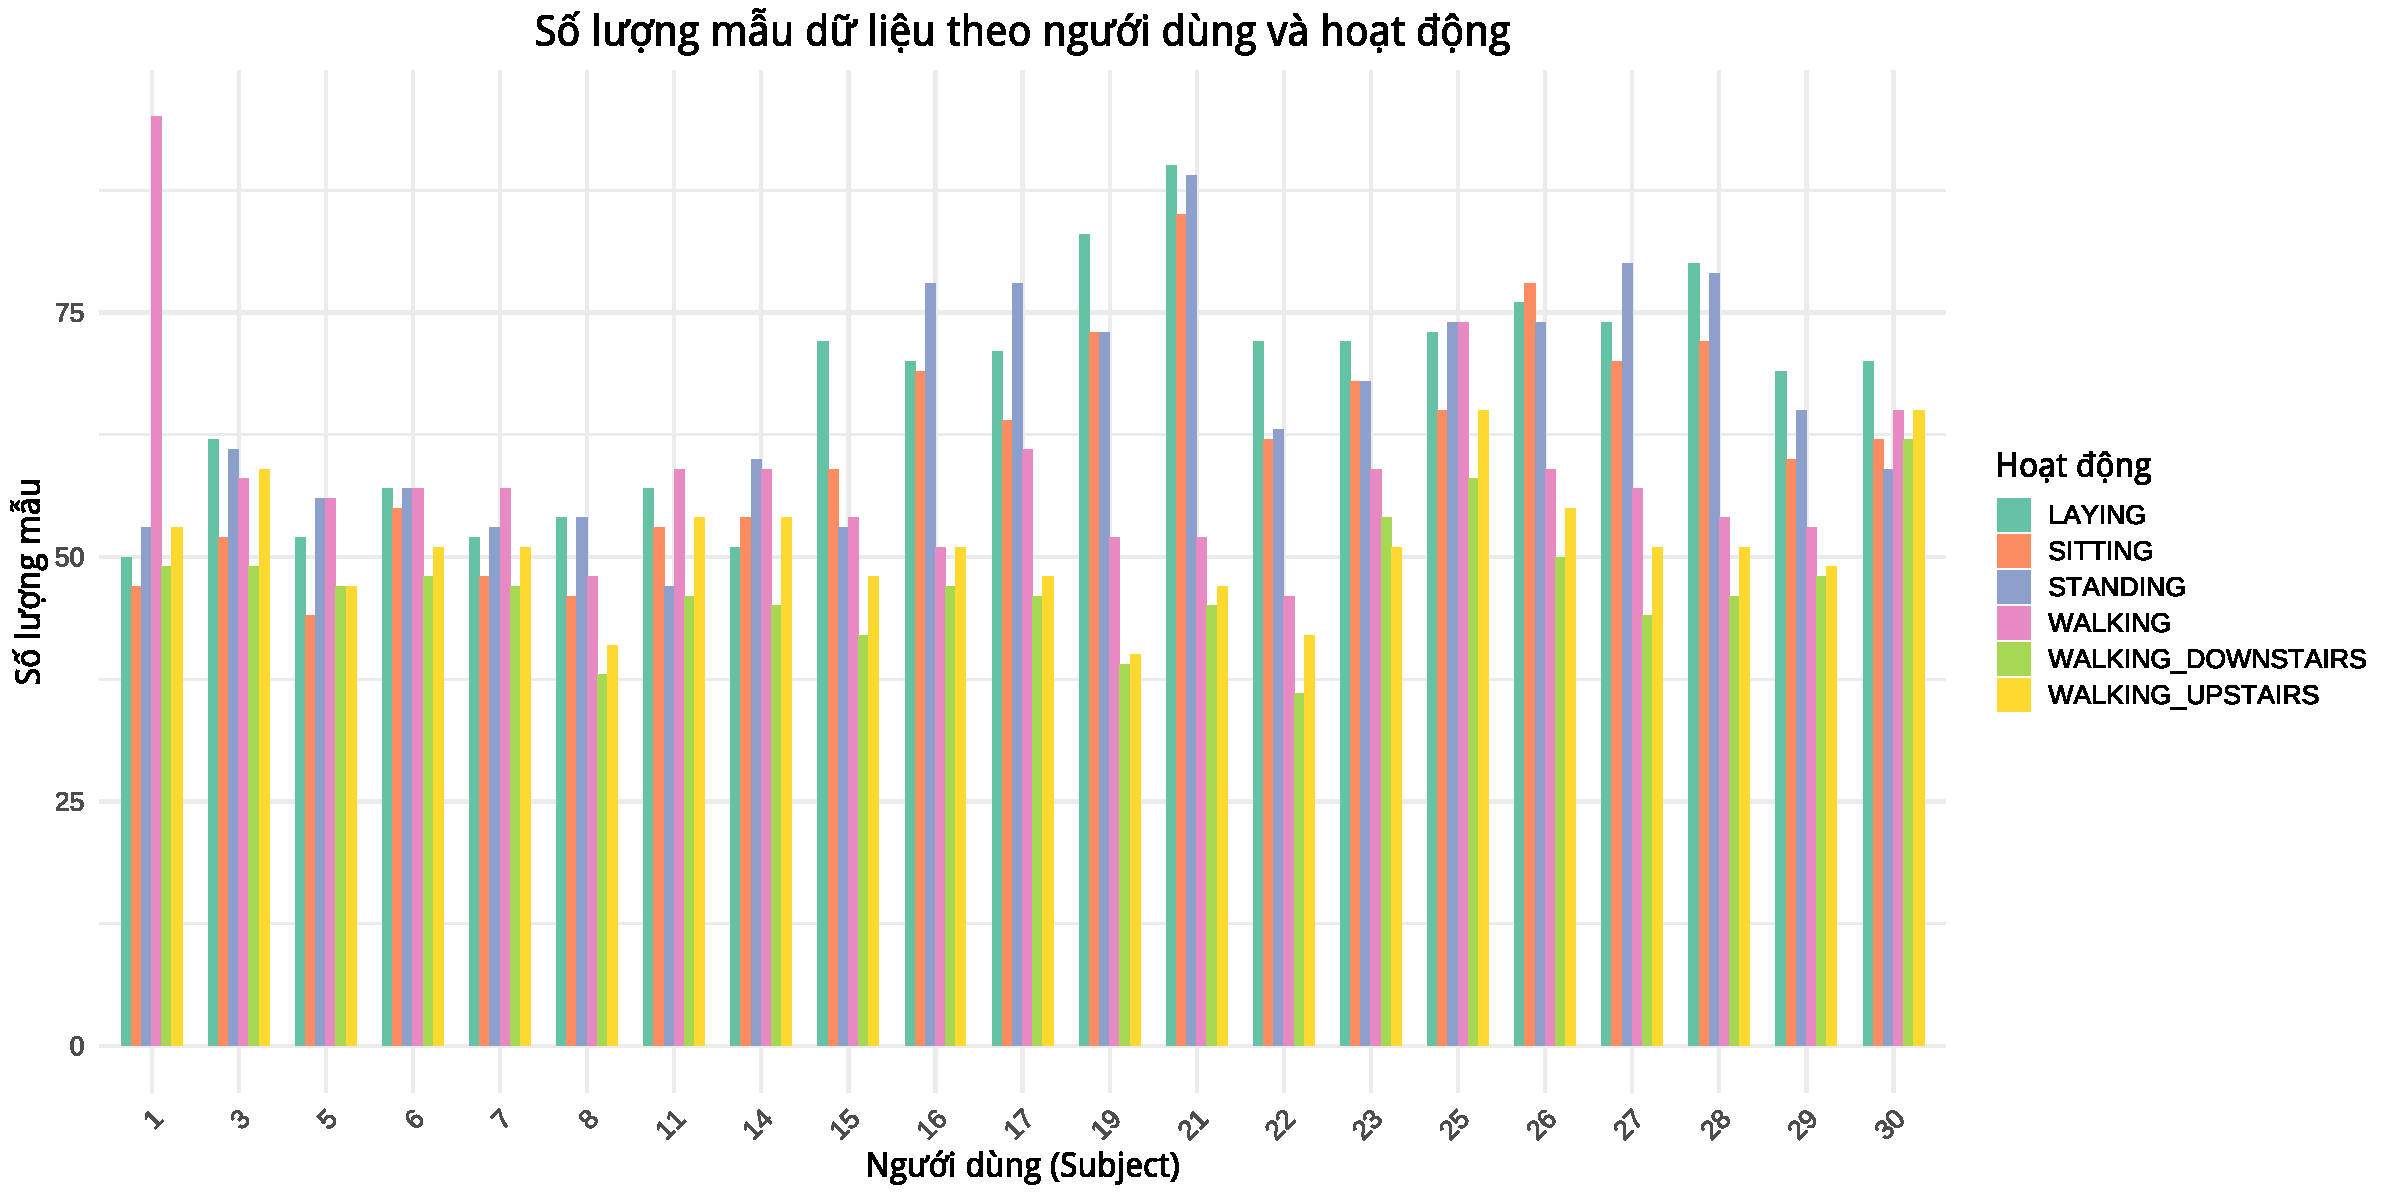
\includegraphics{report_files/figure-latex/unnamed-chunk-11-1.pdf}
\caption{Số lượng mẫu dữ liệu theo người dùng và hoạt động}
\end{figure}

\begin{Shaded}
\begin{Highlighting}[]
\FunctionTok{library}\NormalTok{(ggplot2)}

\FunctionTok{ggplot}\NormalTok{(train, }\FunctionTok{aes}\NormalTok{(}\AttributeTok{x =}\NormalTok{ Activity, }\AttributeTok{fill =}\NormalTok{ Activity)) }\SpecialCharTok{+}
  \FunctionTok{geom\_bar}\NormalTok{() }\SpecialCharTok{+}
  \FunctionTok{labs}\NormalTok{(}
    \AttributeTok{title =} \StringTok{"Số lượng mẫu theo từng hoạt động"}\NormalTok{,}
    \AttributeTok{x =} \StringTok{"Hoạt động"}\NormalTok{,}
    \AttributeTok{y =} \StringTok{"Số lượng mẫu"}
\NormalTok{  ) }\SpecialCharTok{+}
  \FunctionTok{theme\_minimal}\NormalTok{(}\AttributeTok{base\_size =} \DecValTok{15}\NormalTok{) }\SpecialCharTok{+}
  \FunctionTok{theme}\NormalTok{(}
    \AttributeTok{axis.text.x =} \FunctionTok{element\_text}\NormalTok{(}\AttributeTok{angle =} \DecValTok{45}\NormalTok{, }\AttributeTok{vjust =} \DecValTok{1}\NormalTok{, }\AttributeTok{hjust=}\DecValTok{1}\NormalTok{),}
    \AttributeTok{plot.title =} \FunctionTok{element\_text}\NormalTok{(}\AttributeTok{hjust =} \FloatTok{0.5}\NormalTok{, }\AttributeTok{face =} \StringTok{"bold"}\NormalTok{)}
\NormalTok{  ) }\SpecialCharTok{+}
  \FunctionTok{guides}\NormalTok{(}\AttributeTok{fill =} \StringTok{"none"}\NormalTok{)}
\end{Highlighting}
\end{Shaded}

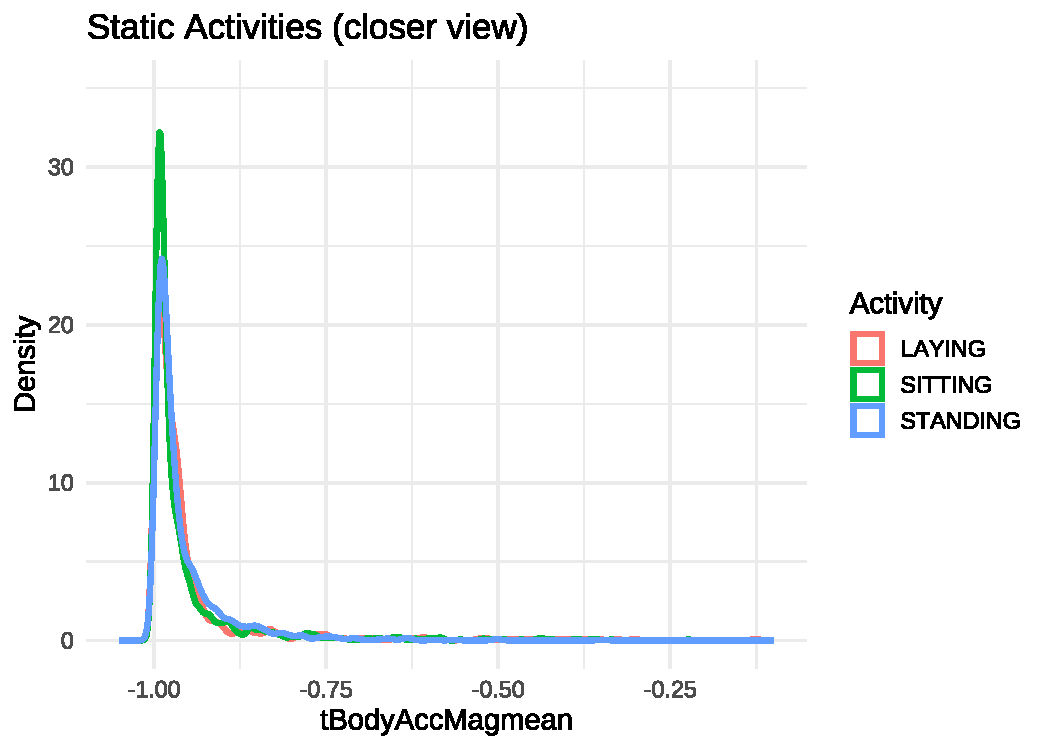
\includegraphics{report_files/figure-latex/unnamed-chunk-12-1.pdf} Số
lượng mẫu cho mỗi hoạt động dao động trong khoảng 1000 mẫu đến 1200 mẫu.
Các hoạt động tĩnh như laying, sitting, standing có xu hướng chiếm tỷ lệ
cao hơn một chút so với các hoạt động di chuyển như walking,
walking\_upstairs, walking\_downstairs. Mức độ chênh lệch không qua lớn
giữa các nhóm, là điểm thuận lợi cho các mô hình học máy tránh bị lệch
nhãn và đảm bảo khả năng học đều giữa các lớp.

\begin{Shaded}
\begin{Highlighting}[]
\FunctionTok{library}\NormalTok{(ggplot2)}

\FunctionTok{ggplot}\NormalTok{(train, }\FunctionTok{aes}\NormalTok{(}\AttributeTok{x =}\NormalTok{ tBodyAccMagmean, }\AttributeTok{color =}\NormalTok{ Activity)) }\SpecialCharTok{+}
  \FunctionTok{geom\_density}\NormalTok{(}\AttributeTok{size =} \FloatTok{1.2}\NormalTok{) }\SpecialCharTok{+}
  \FunctionTok{scale\_color\_brewer}\NormalTok{(}\AttributeTok{palette =} \StringTok{"Set1"}\NormalTok{) }\SpecialCharTok{+}
  \FunctionTok{scale\_x\_continuous}\NormalTok{(}\AttributeTok{limits =} \FunctionTok{c}\NormalTok{(}\SpecialCharTok{{-}}\FloatTok{1.1}\NormalTok{, }\DecValTok{1}\NormalTok{)) }\SpecialCharTok{+} 
  \FunctionTok{labs}\NormalTok{(}
    \AttributeTok{title =} \StringTok{"Phân bố tBodyAccMagmean theo hoạt động"}\NormalTok{,}
    \AttributeTok{x =} \StringTok{"tBodyAccMagmean"}\NormalTok{,}
    \AttributeTok{y =} \StringTok{"Mật độ"}
\NormalTok{  ) }\SpecialCharTok{+}
  \FunctionTok{theme\_minimal}\NormalTok{(}\AttributeTok{base\_size =} \DecValTok{16}\NormalTok{) }\SpecialCharTok{+}
  \FunctionTok{theme}\NormalTok{(}
    \AttributeTok{plot.title =} \FunctionTok{element\_text}\NormalTok{(}\AttributeTok{hjust =} \FloatTok{0.5}\NormalTok{)}
\NormalTok{  )}
\end{Highlighting}
\end{Shaded}

\begin{verbatim}
## Warning: Using `size` aesthetic for lines was deprecated in ggplot2 3.4.0.
## i Please use `linewidth` instead.
## This warning is displayed once every 8 hours.
## Call `lifecycle::last_lifecycle_warnings()` to see where this warning was
## generated.
\end{verbatim}

\begin{figure}
\centering
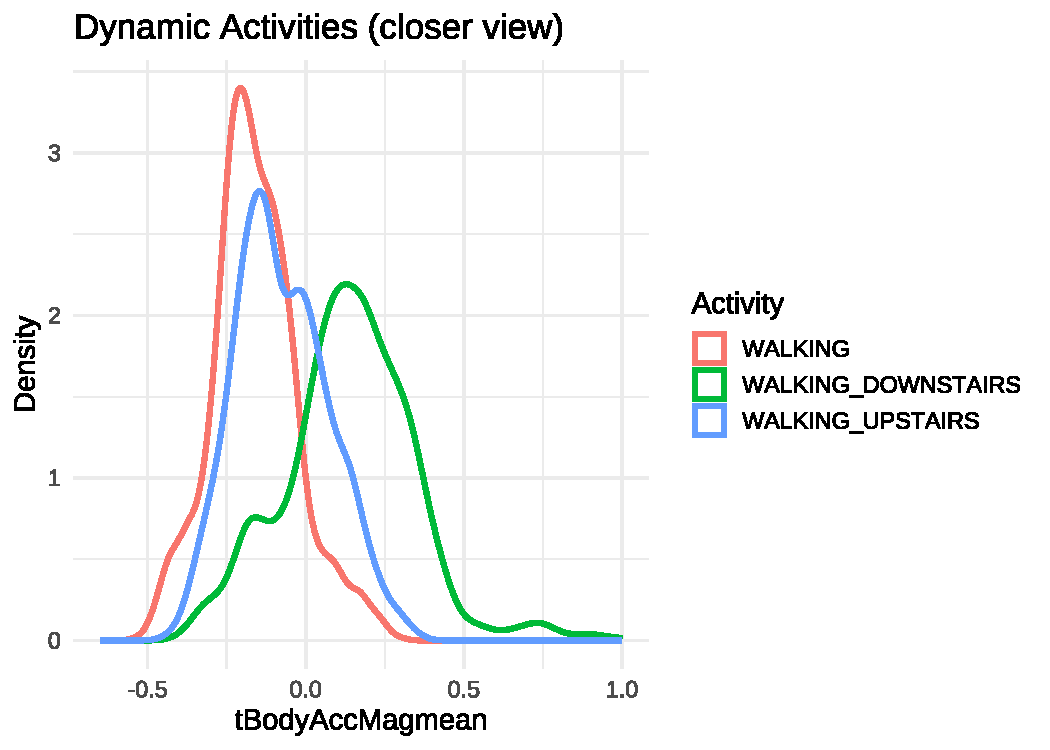
\includegraphics{report_files/figure-latex/unnamed-chunk-13-1.pdf}
\caption{Phân bố tBodyAccMagmean theo hoạt động}
\end{figure}

\begin{Shaded}
\begin{Highlighting}[]
\FunctionTok{library}\NormalTok{(ggplot2)}
\FunctionTok{library}\NormalTok{(dplyr)}
\end{Highlighting}
\end{Shaded}

\begin{verbatim}
## 
## Attaching package: 'dplyr'
\end{verbatim}

\begin{verbatim}
## The following objects are masked from 'package:stats':
## 
##     filter, lag
\end{verbatim}

\begin{verbatim}
## The following objects are masked from 'package:base':
## 
##     intersect, setdiff, setequal, union
\end{verbatim}

\begin{Shaded}
\begin{Highlighting}[]
\FunctionTok{library}\NormalTok{(gridExtra)}
\end{Highlighting}
\end{Shaded}

\begin{verbatim}
## 
## Attaching package: 'gridExtra'
\end{verbatim}

\begin{verbatim}
## The following object is masked from 'package:dplyr':
## 
##     combine
\end{verbatim}

\begin{Shaded}
\begin{Highlighting}[]
\NormalTok{p1 }\OtherTok{\textless{}{-}}\NormalTok{ train }\SpecialCharTok{\%\textgreater{}\%}
  \FunctionTok{filter}\NormalTok{(Activity }\SpecialCharTok{\%in\%} \FunctionTok{c}\NormalTok{(}\StringTok{"SITTING"}\NormalTok{, }\StringTok{"STANDING"}\NormalTok{, }\StringTok{"LAYING"}\NormalTok{)) }\SpecialCharTok{\%\textgreater{}\%}
  \FunctionTok{ggplot}\NormalTok{(}\FunctionTok{aes}\NormalTok{(}\AttributeTok{x =}\NormalTok{ tBodyAccMagmean, }\AttributeTok{color =}\NormalTok{ Activity)) }\SpecialCharTok{+}
  \FunctionTok{geom\_density}\NormalTok{(}\AttributeTok{size =} \FloatTok{1.2}\NormalTok{) }\SpecialCharTok{+}
  \FunctionTok{labs}\NormalTok{(}
    \AttributeTok{title =} \StringTok{"Static Activities (closer view)"}\NormalTok{,}
    \AttributeTok{x =} \StringTok{"tBodyAccMagmean"}\NormalTok{,}
    \AttributeTok{y =} \StringTok{"Density"}
\NormalTok{  ) }\SpecialCharTok{+}
  \FunctionTok{xlim}\NormalTok{(}\SpecialCharTok{{-}}\FloatTok{1.05}\NormalTok{, }\SpecialCharTok{{-}}\FloatTok{0.1}\NormalTok{) }\SpecialCharTok{+}
  \FunctionTok{ylim}\NormalTok{(}\DecValTok{0}\NormalTok{, }\DecValTok{35}\NormalTok{) }\SpecialCharTok{+}
  \FunctionTok{theme\_minimal}\NormalTok{(}\AttributeTok{base\_size =} \DecValTok{14}\NormalTok{)}
\NormalTok{p1}
\end{Highlighting}
\end{Shaded}

\begin{figure}
\centering
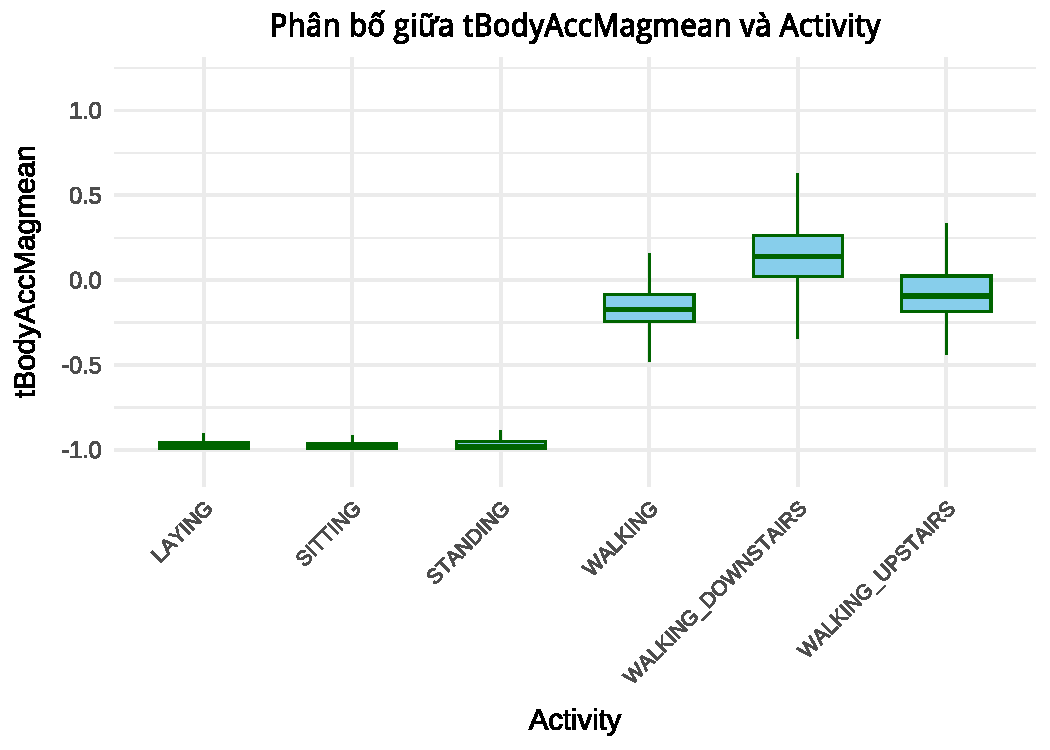
\includegraphics{report_files/figure-latex/unnamed-chunk-14-1.pdf}
\caption{Phân bố tBodyAccMagmean theo hoạt động sitting, standing,
laying}
\end{figure}

\begin{Shaded}
\begin{Highlighting}[]
\NormalTok{p2 }\OtherTok{\textless{}{-}}\NormalTok{ train }\SpecialCharTok{\%\textgreater{}\%}
  \FunctionTok{filter}\NormalTok{(Activity }\SpecialCharTok{\%in\%} \FunctionTok{c}\NormalTok{(}\StringTok{"WALKING"}\NormalTok{, }\StringTok{"WALKING\_DOWNSTAIRS"}\NormalTok{, }\StringTok{"WALKING\_UPSTAIRS"}\NormalTok{)) }\SpecialCharTok{\%\textgreater{}\%}
  \FunctionTok{ggplot}\NormalTok{(}\FunctionTok{aes}\NormalTok{(}\AttributeTok{x =}\NormalTok{ tBodyAccMagmean, }\AttributeTok{color =}\NormalTok{ Activity)) }\SpecialCharTok{+}
  \FunctionTok{geom\_density}\NormalTok{(}\AttributeTok{size =} \FloatTok{1.2}\NormalTok{) }\SpecialCharTok{+}
  \FunctionTok{labs}\NormalTok{(}
    \AttributeTok{title =} \StringTok{"Dynamic Activities (closer view)"}\NormalTok{,}
    \AttributeTok{x =} \StringTok{"tBodyAccMagmean"}\NormalTok{,}
    \AttributeTok{y =} \StringTok{"Density"}
\NormalTok{  ) }\SpecialCharTok{+} \FunctionTok{xlim}\NormalTok{(}\SpecialCharTok{{-}}\FloatTok{0.65}\NormalTok{, }\DecValTok{1}\NormalTok{) }\SpecialCharTok{+}
  \FunctionTok{theme\_minimal}\NormalTok{(}\AttributeTok{base\_size =} \DecValTok{14}\NormalTok{)}

\NormalTok{p2}
\end{Highlighting}
\end{Shaded}

\begin{figure}
\centering
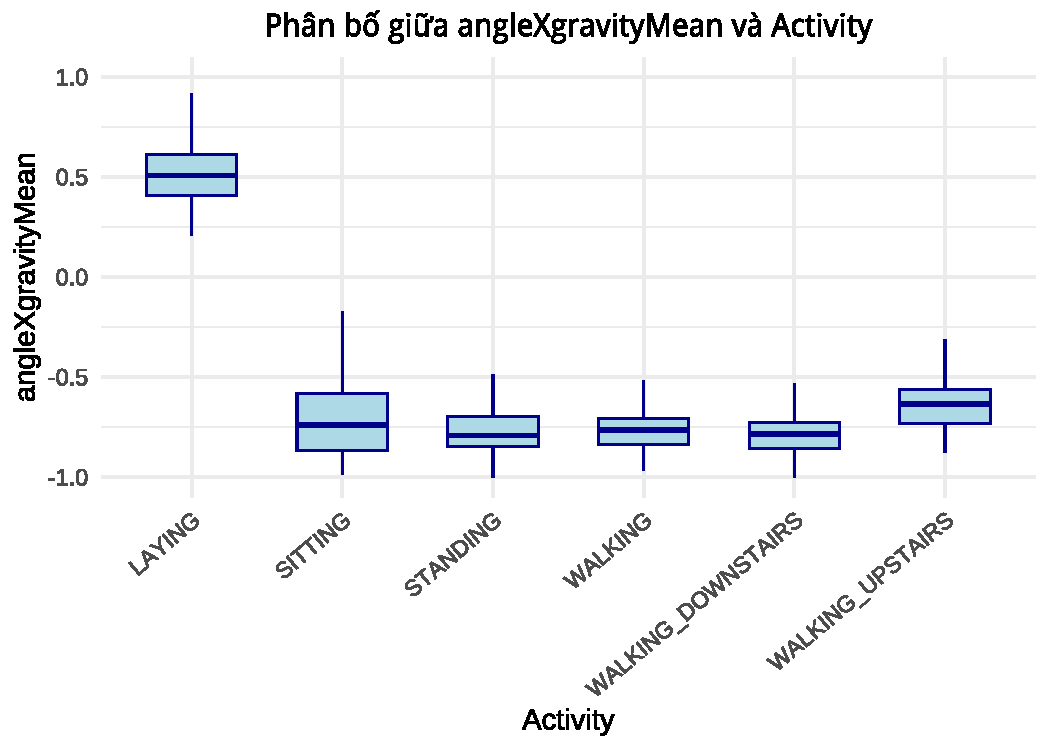
\includegraphics{report_files/figure-latex/unnamed-chunk-15-1.pdf}
\caption{Phân bố tBodyAccMagmean theo hoạt động walking,
walking\_dowstairs, walking\_upstairs}
\end{figure}

\begin{Shaded}
\begin{Highlighting}[]
\FunctionTok{library}\NormalTok{(ggplot2)}

\FunctionTok{ggplot}\NormalTok{(train, }\FunctionTok{aes}\NormalTok{(}\AttributeTok{x =}\NormalTok{ Activity, }\AttributeTok{y =}\NormalTok{ tBodyAccMagmean)) }\SpecialCharTok{+}
  \FunctionTok{geom\_boxplot}\NormalTok{(}
    \AttributeTok{outlier.shape =} \ConstantTok{NA}\NormalTok{,}
    \AttributeTok{fill =} \StringTok{"skyblue"}\NormalTok{,}
    \AttributeTok{color =} \StringTok{"darkgreen"}\NormalTok{,}
    \AttributeTok{width =} \FloatTok{0.6}
\NormalTok{  ) }\SpecialCharTok{+}
  \FunctionTok{labs}\NormalTok{(}
    \AttributeTok{title =} \StringTok{"Phân bố giữa tBodyAccMagmean và Activity"}\NormalTok{,}
    \AttributeTok{y =} \StringTok{"tBodyAccMagmean"}\NormalTok{,}
    \AttributeTok{x =} \StringTok{"Activity"}
\NormalTok{  ) }\SpecialCharTok{+}
  \FunctionTok{coord\_cartesian}\NormalTok{(}\AttributeTok{ylim =} \FunctionTok{c}\NormalTok{(}\SpecialCharTok{{-}}\FloatTok{1.1}\NormalTok{, }\FloatTok{1.2}\NormalTok{)) }\SpecialCharTok{+} 
  \FunctionTok{theme\_minimal}\NormalTok{(}\AttributeTok{base\_size =} \DecValTok{14}\NormalTok{) }\SpecialCharTok{+}
  \FunctionTok{theme}\NormalTok{(}
    \AttributeTok{plot.title =} \FunctionTok{element\_text}\NormalTok{(}\AttributeTok{hjust =} \FloatTok{0.5}\NormalTok{, }\AttributeTok{size =} \DecValTok{15}\NormalTok{, }\AttributeTok{face =} \StringTok{"bold"}\NormalTok{),}
    \AttributeTok{axis.text.x =} \FunctionTok{element\_text}\NormalTok{(}\AttributeTok{angle =} \DecValTok{45}\NormalTok{, }\AttributeTok{hjust =} \DecValTok{1}\NormalTok{, }\AttributeTok{size =} \DecValTok{10}\NormalTok{),}
    \AttributeTok{axis.title.x =} \FunctionTok{element\_text}\NormalTok{(}\AttributeTok{margin =} \FunctionTok{margin}\NormalTok{(}\AttributeTok{t =} \DecValTok{10}\NormalTok{)),}
    \AttributeTok{axis.title.y =} \FunctionTok{element\_text}\NormalTok{(}\AttributeTok{margin =} \FunctionTok{margin}\NormalTok{(}\AttributeTok{r =} \DecValTok{10}\NormalTok{))}
\NormalTok{  )}
\end{Highlighting}
\end{Shaded}

\begin{figure}
\centering
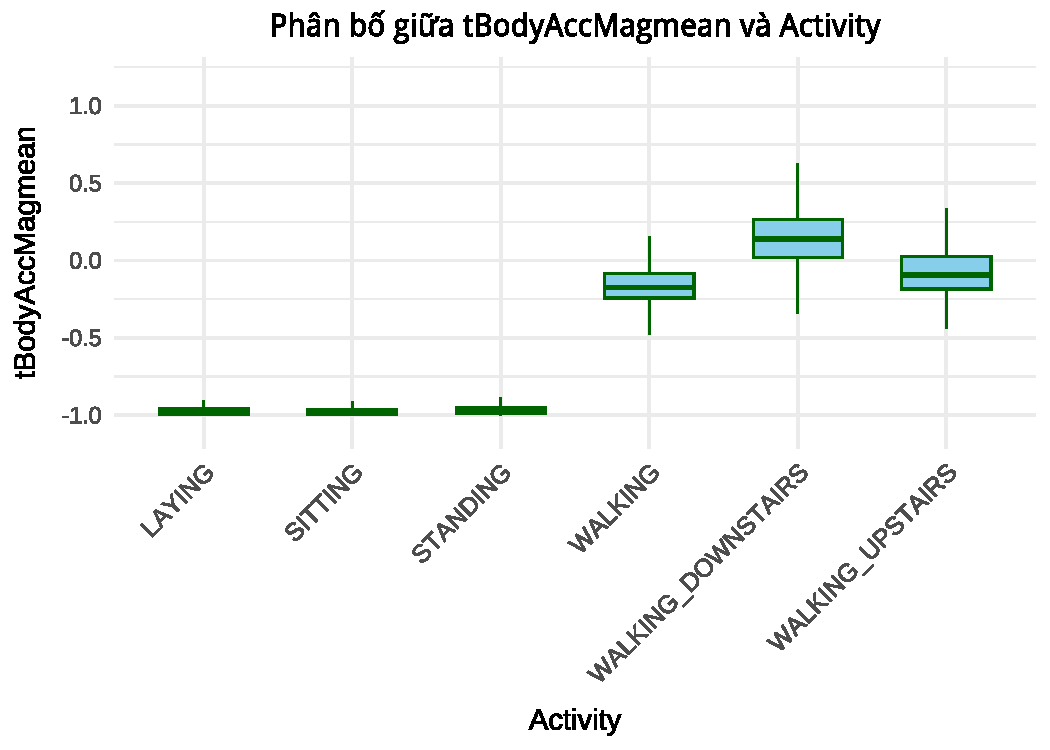
\includegraphics{report_files/figure-latex/unnamed-chunk-16-1.pdf}
\caption{Phân bố giữa tBodyAccMagmean và Activity}
\end{figure}

\begin{Shaded}
\begin{Highlighting}[]
\FunctionTok{library}\NormalTok{(ggplot2)}

\FunctionTok{ggplot}\NormalTok{(train, }\FunctionTok{aes}\NormalTok{(}\AttributeTok{x =}\NormalTok{ Activity, }\AttributeTok{y =}\NormalTok{ angleXgravityMean)) }\SpecialCharTok{+}
  \FunctionTok{geom\_boxplot}\NormalTok{(}
    \AttributeTok{fill =} \StringTok{"lightblue"}\NormalTok{,}
    \AttributeTok{color =} \StringTok{"darkblue"}\NormalTok{,}
    \AttributeTok{outlier.shape =} \ConstantTok{NA}\NormalTok{,}
    \AttributeTok{width =} \FloatTok{0.6}
\NormalTok{  ) }\SpecialCharTok{+}
  \FunctionTok{labs}\NormalTok{(}
    \AttributeTok{title =} \StringTok{"Phân bố giữa angleXgravityMean và Activity"}\NormalTok{,}
    \AttributeTok{x =} \StringTok{"Activity"}\NormalTok{,}
    \AttributeTok{y =} \StringTok{"angleXgravityMean"}
\NormalTok{  ) }\SpecialCharTok{+}
  \FunctionTok{theme\_minimal}\NormalTok{(}\AttributeTok{base\_size =} \DecValTok{14}\NormalTok{) }\SpecialCharTok{+}
  \FunctionTok{theme}\NormalTok{(}
    \AttributeTok{plot.title =} \FunctionTok{element\_text}\NormalTok{(}\AttributeTok{hjust =} \FloatTok{0.5}\NormalTok{, }\AttributeTok{size =} \DecValTok{15}\NormalTok{, }\AttributeTok{face =} \StringTok{"bold"}\NormalTok{),}
    \AttributeTok{axis.text.x =} \FunctionTok{element\_text}\NormalTok{(}\AttributeTok{angle =} \DecValTok{40}\NormalTok{, }\AttributeTok{hjust =} \DecValTok{1}\NormalTok{, }\AttributeTok{size =} \DecValTok{11}\NormalTok{)}
\NormalTok{  )}
\end{Highlighting}
\end{Shaded}

\begin{figure}
\centering
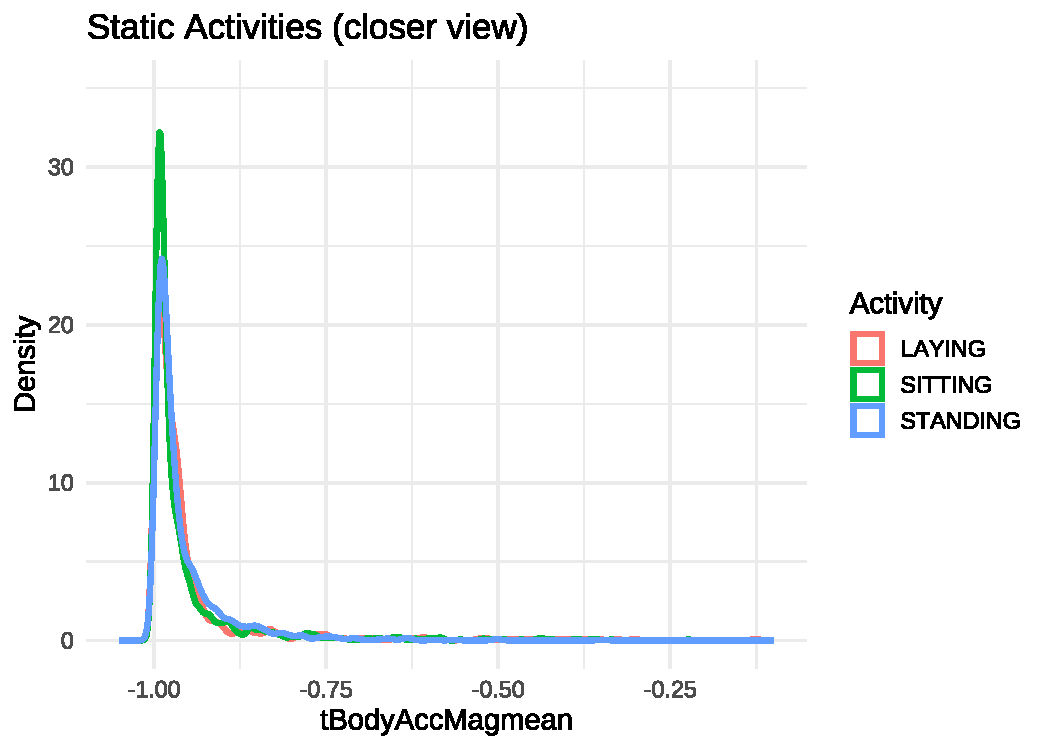
\includegraphics{report_files/figure-latex/unnamed-chunk-17-1.pdf}
\caption{Phân bố giữa angleXgravityMean và Activity}
\end{figure}

\begin{Shaded}
\begin{Highlighting}[]
\FunctionTok{library}\NormalTok{(ggplot2)}

\FunctionTok{ggplot}\NormalTok{(train, }\FunctionTok{aes}\NormalTok{(}\AttributeTok{x =}\NormalTok{ Activity, }\AttributeTok{y =}\NormalTok{ angleYgravityMean)) }\SpecialCharTok{+}
  \FunctionTok{geom\_boxplot}\NormalTok{(}
    \AttributeTok{fill =} \StringTok{"lightblue"}\NormalTok{,}
    \AttributeTok{color =} \StringTok{"darkblue"}\NormalTok{,}
    \AttributeTok{outlier.shape =} \ConstantTok{NA}\NormalTok{,}
    \AttributeTok{width =} \FloatTok{0.6}
\NormalTok{  ) }\SpecialCharTok{+}
  \FunctionTok{labs}\NormalTok{(}
    \AttributeTok{title =} \StringTok{"Phân bố giữa angleYgravityMean và Activity"}\NormalTok{,}
    \AttributeTok{x =} \StringTok{"Activity"}\NormalTok{,}
    \AttributeTok{y =} \StringTok{"angleYgravityMean"}
\NormalTok{  ) }\SpecialCharTok{+}
  \FunctionTok{theme\_minimal}\NormalTok{(}\AttributeTok{base\_size =} \DecValTok{14}\NormalTok{) }\SpecialCharTok{+}
  \FunctionTok{theme}\NormalTok{(}
    \AttributeTok{plot.title =} \FunctionTok{element\_text}\NormalTok{(}\AttributeTok{hjust =} \FloatTok{0.5}\NormalTok{, }\AttributeTok{size =} \DecValTok{15}\NormalTok{, }\AttributeTok{face =} \StringTok{"bold"}\NormalTok{),}
    \AttributeTok{axis.text.x =} \FunctionTok{element\_text}\NormalTok{(}\AttributeTok{angle =} \DecValTok{40}\NormalTok{, }\AttributeTok{hjust =} \DecValTok{1}\NormalTok{, }\AttributeTok{size =} \DecValTok{11}\NormalTok{)}
\NormalTok{  )}
\end{Highlighting}
\end{Shaded}

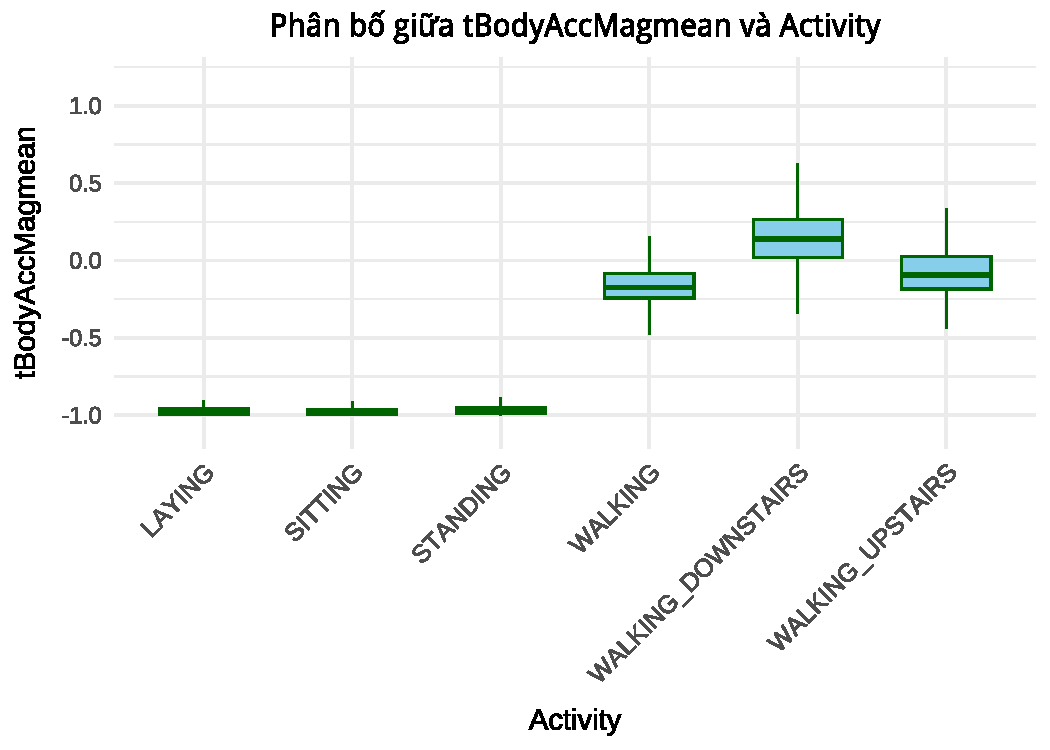
\includegraphics{report_files/figure-latex/unnamed-chunk-18-1.pdf}

Đặc trưng tBodyAccMagmean -- đại diện cho độ lớn trung bình của gia tốc
cơ thể trong mỗi phân đoạn tín hiệu. Biểu đồ mật độ cho thấy ba hoạt
động tĩnh đều có phân phối rất hẹp, tập trung gần giá trị -1.0, với đỉnh
phân phối cao và sắc. Điều này phản ánh rằng khi người dùng không di
chuyển, thiết bị ở thắt lưng ghi nhận gia tốc gần như bằng 0 trong toàn
bộ cửa sổ thời gian. Trong đó, hoạt động SITTING có mật độ tập trung cao
nhất, cho thấy đây là tư thế có ít dao động nhất; STANDING có phân bố
hơi rộng hơn một chút, có thể do người thực hiện có xu hướng chuyển
trọng lượng nhẹ nhàng khi đứng. Ngược lại, hoạt động LAYING lại xuất
hiện sự phân tán hơn -- phản ánh trạng thái nằm có thể mang nhiều tư thế
khác nhau (nằm nghiêng, nằm ngửa\ldots).

AngleXgravityMean cho thấy sự khác biệt rõ giữa tư thế nằm và các tư thế
còn lại: trong khi LAYING có giá trị trung bình dương lớn (≈ 0.5--0.7),
các hoạt động khác có xu hướng âm rõ rệt, thường nằm trong khoảng -0.6
đến -1.0. Là chỉ báo mạnh về góc nghiêng của cơ thể theo trục
trước--sau, rất hữu ích trong việc phân biệt trạng thái nghỉ ngơi so với
trạng thái hoạt động.

AngleYgravityMean -- thể hiện góc nghiêng cơ thể theo trục ngang. LAYING
có giá trị âm lớn (≈ -0.5), SITTING nằm quanh giá trị 0, trong khi
STANDING và các hoạt động di chuyển đều có giá trị dương và tập trung
gần nhau, phản ánh trạng thái thẳng đứng của cơ thể. Các đặc trưng liên
quan đến góc độ không gian của thiết bị có khả năng phân biệt rõ tư thế
mà không cần đến các đặc trưng vận tốc hay gia tốc.

Phân tích các đặc trưng tBodyAccMagmean, angleXgravityMean và
angleYgravityMean không chỉ làm rõ cấu trúc phân bố của dữ liệu, mà còn
cho thấy mỗi hoạt động trong bộ dữ liệu HAR đều thể hiện dấu hiệu đặc
trưng về mặt hình học hoặc vận động học, đóng vai trò quan trọng trong
việc xây dựng các mô hình học máy chính xác nhằm phân loại hành vi người
dùng.

\section*{CHƯƠNG 4: THỰC NGHIỆM}
\addcontentsline{toc}{section}{CHƯƠNG 4: THỰC NGHIỆM}
\setcounter{section}{4}
\setcounter{subsection}{0}

\subsection{Kiểm tra outlier}\label{kiux1ec3m-tra-outlier}

Tiến hành kiểm tra outlier trên tập train và tập test, xác định các điểm
ngoại lai bằng phương pháp khoảng tứ phân vị (Interquartile Range --
IQR). Loại bỏ biến subject và Activity để tạo ra tập dữ liệu
sensor\_data, bao gồm 561 đặc trưng cảm biến, với mỗi cột trong tập dữ
liệu xác định ranh giới bất thường dựa trên công thức: \[
\text{Lower bound} = Q1 - 1.5 \times IQR, \quad
\text{Upper bound} = Q3 + 1.5 \times IQR
\] Trong đó \emph{\(Q1\)} và \emph{\(Q3\)} là các tứ phân vị thứ nhất và
thứ ba tương ứng, và \emph{\(IQR = Q3 - Q1\)}. Mọi giá trị vượt ngoài
khoảng này được coi là ngoại lai.

\begin{Shaded}
\begin{Highlighting}[]
\NormalTok{subject\_ids }\OtherTok{\textless{}{-}}\NormalTok{ train}\SpecialCharTok{$}\NormalTok{subject}
\NormalTok{activity\_labels }\OtherTok{\textless{}{-}}\NormalTok{ train}\SpecialCharTok{$}\NormalTok{Activity}
\NormalTok{sensor\_data }\OtherTok{\textless{}{-}}\NormalTok{ train[, }\SpecialCharTok{!}\NormalTok{(}\FunctionTok{names}\NormalTok{(train) }\SpecialCharTok{\%in\%} \FunctionTok{c}\NormalTok{(}\StringTok{"Activity"}\NormalTok{, }\StringTok{"subject"}\NormalTok{))]}
\NormalTok{subject\_ids\_test }\OtherTok{\textless{}{-}}\NormalTok{ test}\SpecialCharTok{$}\NormalTok{subject}
\NormalTok{activity\_labels\_test }\OtherTok{\textless{}{-}}\NormalTok{ test}\SpecialCharTok{$}\NormalTok{Activity}
\NormalTok{sensor\_data\_test }\OtherTok{\textless{}{-}}\NormalTok{ test[, }\SpecialCharTok{!}\NormalTok{(}\FunctionTok{names}\NormalTok{(test) }\SpecialCharTok{\%in\%} \FunctionTok{c}\NormalTok{(}\StringTok{"Activity"}\NormalTok{, }\StringTok{"subject"}\NormalTok{))]}

\NormalTok{is\_outlier\_iqr }\OtherTok{\textless{}{-}} \ControlFlowTok{function}\NormalTok{(x) \{}
\NormalTok{  Q1 }\OtherTok{\textless{}{-}} \FunctionTok{quantile}\NormalTok{(x, }\FloatTok{0.25}\NormalTok{, }\AttributeTok{na.rm =} \ConstantTok{TRUE}\NormalTok{)}
\NormalTok{  Q3 }\OtherTok{\textless{}{-}} \FunctionTok{quantile}\NormalTok{(x, }\FloatTok{0.75}\NormalTok{, }\AttributeTok{na.rm =} \ConstantTok{TRUE}\NormalTok{)}
\NormalTok{  IQR\_val }\OtherTok{\textless{}{-}}\NormalTok{ Q3 }\SpecialCharTok{{-}}\NormalTok{ Q1}
\NormalTok{  lower\_bound }\OtherTok{\textless{}{-}}\NormalTok{ Q1 }\SpecialCharTok{{-}} \FloatTok{1.5} \SpecialCharTok{*}\NormalTok{ IQR\_val}
\NormalTok{  upper\_bound }\OtherTok{\textless{}{-}}\NormalTok{ Q3 }\SpecialCharTok{+} \FloatTok{1.5} \SpecialCharTok{*}\NormalTok{ IQR\_val}
\NormalTok{  x }\SpecialCharTok{\textless{}}\NormalTok{ lower\_bound }\SpecialCharTok{|}\NormalTok{ x }\SpecialCharTok{\textgreater{}}\NormalTok{ upper\_bound}
\NormalTok{\}}

\NormalTok{outlier\_matrix }\OtherTok{\textless{}{-}} \FunctionTok{mapply}\NormalTok{(is\_outlier\_iqr, sensor\_data)}

\NormalTok{total\_outlier\_values }\OtherTok{\textless{}{-}} \FunctionTok{sum}\NormalTok{(outlier\_matrix)}
\NormalTok{total\_cells }\OtherTok{\textless{}{-}} \FunctionTok{nrow}\NormalTok{(sensor\_data) }\SpecialCharTok{*} \FunctionTok{ncol}\NormalTok{(sensor\_data)}
\NormalTok{percent\_outlier\_cells }\OtherTok{\textless{}{-}} \FunctionTok{round}\NormalTok{(total\_outlier\_values }\SpecialCharTok{/}\NormalTok{ total\_cells }\SpecialCharTok{*} \DecValTok{100}\NormalTok{, }\DecValTok{2}\NormalTok{)}

\FunctionTok{cat}\NormalTok{(}\StringTok{"Tổng số giá trị outlier:"}\NormalTok{, total\_outlier\_values, }\StringTok{"/"}\NormalTok{, total\_cells, }\StringTok{"}\SpecialCharTok{\textbackslash{}n}\StringTok{"}\NormalTok{)}
\end{Highlighting}
\end{Shaded}

\begin{verbatim}
## Tổng số giá trị outlier: 163682 / 4124472
\end{verbatim}

\begin{Shaded}
\begin{Highlighting}[]
\FunctionTok{cat}\NormalTok{(}\StringTok{"Tỷ lệ giá trị outlier:"}\NormalTok{, percent\_outlier\_cells, }\StringTok{"\%}\SpecialCharTok{\textbackslash{}n}\StringTok{"}\NormalTok{)}
\end{Highlighting}
\end{Shaded}

\begin{verbatim}
## Tỷ lệ giá trị outlier: 3.97 %
\end{verbatim}

Kết quả có tổng cộng 163,682 giá trị được đánh dấu là ngoại lai, trên
tổng số 4,124,472 giá trị dữ liệu. Điều này tương ứng với tỷ lệ 3.97\%,
một mức thấp, dữ liệu phần lớn ổn định và sạch.

\begin{itemize}
\tightlist
\item
  Tiến hành Chuẩn hóa outlier bằng kỹ thuật cắt ngưỡng (Percentile
  Capping) nhằm giảm ảnh hưởng của các outlier mà không loại bỏ chúng
  hoàn toàn khỏi tập dữ liệu. Thay thế các giá trị cực đoan bằng một
  ngưỡng giới hạn mềm dựa trên các phân vị phần trăm (percentiles) của
  phân phối dữ liệu. định nghĩa một hàm cap\_outliers() để áp dụng quy
  tắc sau trên từng cột trong bảng dữ liệu: giá trị nhỏ hơn phân vị 1\%
  (1st percentile) được gán bằng chính giá trị tại phân vị này, giá trị
  lớn hơn phân vị 99\% (99th percentile) được gán bằng giá trị tại phân
  vị đó, các giá trị nằm giữa hai ngưỡng này được giữ nguyên.
\end{itemize}

\begin{Shaded}
\begin{Highlighting}[]
\NormalTok{ cap\_outliers }\OtherTok{\textless{}{-}} \ControlFlowTok{function}\NormalTok{(df, }\AttributeTok{lower =} \FloatTok{0.01}\NormalTok{, }\AttributeTok{upper =} \FloatTok{0.99}\NormalTok{) \{}
   \ControlFlowTok{for}\NormalTok{ (col }\ControlFlowTok{in} \FunctionTok{names}\NormalTok{(df)) \{}
\NormalTok{     q\_low }\OtherTok{\textless{}{-}} \FunctionTok{quantile}\NormalTok{(df[[col]], lower, }\AttributeTok{na.rm =} \ConstantTok{TRUE}\NormalTok{)}
\NormalTok{     q\_high }\OtherTok{\textless{}{-}} \FunctionTok{quantile}\NormalTok{(df[[col]], upper, }\AttributeTok{na.rm =} \ConstantTok{TRUE}\NormalTok{)}
\NormalTok{     df[[col]] }\OtherTok{\textless{}{-}} \FunctionTok{pmin}\NormalTok{(}\FunctionTok{pmax}\NormalTok{(df[[col]], q\_low), q\_high)}
\NormalTok{   \}}
\NormalTok{   df}
\NormalTok{ \}}

\NormalTok{ sensor\_data\_capped }\OtherTok{\textless{}{-}} \FunctionTok{cap\_outliers}\NormalTok{(sensor\_data)}
\NormalTok{ sensor\_data\_test\_capped }\OtherTok{\textless{}{-}} \FunctionTok{cap\_outliers}\NormalTok{(sensor\_data\_test)}

\NormalTok{ train\_capped }\OtherTok{\textless{}{-}} \FunctionTok{cbind}\NormalTok{(sensor\_data\_capped, }\AttributeTok{subject =}\NormalTok{ subject\_ids, }\AttributeTok{Activity =}\NormalTok{ activity\_labels)}
\NormalTok{ test\_capped }\OtherTok{\textless{}{-}} \FunctionTok{cbind}\NormalTok{(sensor\_data\_test\_capped, }\AttributeTok{subject =}\NormalTok{ subject\_ids\_test, }\AttributeTok{Activity =}\NormalTok{ activity\_labels\_test)}

\CommentTok{\# str(train\_capped)}
\CommentTok{\# str(test\_capped)}
\end{Highlighting}
\end{Shaded}

\subsection{Giảm chiều dữ liệu bằng
UMAP}\label{giux1ea3m-chiux1ec1u-dux1eef-liux1ec7u-bux1eb1ng-umap}

Kỹ thuật UMAP sử dụng để giảm chiều dữ liệu nhằm mục tiêu trực quan hóa
và đánh giá khả năng phân tách giữa các nhãn hoạt động khác nhau. Việc
giảm chiều không gian về 2 chiều giúp quan sát cấu trúc không gian nhúng
của dữ liệu gốc gồm 561 đặc trưng đầu vào. Thử nghiệm hệ thống trên lưới
các tổ hợp siêu tham số khác nhau, số lượng lân cận (n\_neighbors): 5,
15, 30 thể hiện mức độ chú trọng vào cấu trúc cục bộ hay toàn cục. Giá
trị nhỏ nhấn mạnh mối quan hệ địa phương, giá trị lớn mang tính toàn cục
cao hơn. Khoảng cách tối thiểu (min\_dist): 0.001, 0.01, 0.1 điều chỉnh
mức độ nén các cụm dữ liệu trong không gian nhúng. Giá trị càng nhỏ thì
các cụm càng bị nén lại gần nhau, cho phép bảo toàn mật độ; giá trị lớn
làm dàn trải không gian nhúng. Kết quả được trình bày thông qua ma trận
trực quan gồm 9 biểu đồ, tương ứng với 9 tổ hợp siêu tham số khác nhau.
Mỗi điểm trên biểu đồ đại diện cho một mẫu dữ liệu cảm biến, được tô màu
theo nhãn Activity.

\begin{Shaded}
\begin{Highlighting}[]
\FunctionTok{library}\NormalTok{(umap)}
\FunctionTok{library}\NormalTok{(ggplot2)}
\FunctionTok{library}\NormalTok{(gridExtra)}

\NormalTok{perform\_umap\_grid }\OtherTok{\textless{}{-}} \ControlFlowTok{function}\NormalTok{(X\_data, y\_data,}
                              \AttributeTok{neighbors\_list =} \FunctionTok{c}\NormalTok{(}\DecValTok{5}\NormalTok{, }\DecValTok{15}\NormalTok{, }\DecValTok{30}\NormalTok{),}
                              \AttributeTok{min\_dist\_list =} \FunctionTok{c}\NormalTok{(}\FloatTok{0.001}\NormalTok{, }\FloatTok{0.01}\NormalTok{, }\FloatTok{0.1}\NormalTok{)) \{}
\NormalTok{  plots }\OtherTok{\textless{}{-}} \FunctionTok{list}\NormalTok{()}
\NormalTok{  index }\OtherTok{\textless{}{-}} \DecValTok{1}

  \ControlFlowTok{for}\NormalTok{ (n }\ControlFlowTok{in}\NormalTok{ neighbors\_list) \{}
    \ControlFlowTok{for}\NormalTok{ (d }\ControlFlowTok{in}\NormalTok{ min\_dist\_list) \{}
\NormalTok{      config }\OtherTok{\textless{}{-}}\NormalTok{ umap.defaults}
\NormalTok{      config}\SpecialCharTok{$}\NormalTok{n\_neighbors }\OtherTok{\textless{}{-}}\NormalTok{ n}
\NormalTok{      config}\SpecialCharTok{$}\NormalTok{min\_dist }\OtherTok{\textless{}{-}}\NormalTok{ d}
\NormalTok{      config}\SpecialCharTok{$}\NormalTok{n\_components }\OtherTok{\textless{}{-}} \DecValTok{2}

\NormalTok{      umap\_result }\OtherTok{\textless{}{-}} \FunctionTok{umap}\NormalTok{(X\_data, }\AttributeTok{config =}\NormalTok{ config)}
\NormalTok{      df }\OtherTok{\textless{}{-}} \FunctionTok{as.data.frame}\NormalTok{(umap\_result}\SpecialCharTok{$}\NormalTok{layout)}
      \FunctionTok{colnames}\NormalTok{(df) }\OtherTok{\textless{}{-}} \FunctionTok{c}\NormalTok{(}\StringTok{"x"}\NormalTok{, }\StringTok{"y"}\NormalTok{)}
\NormalTok{      df}\SpecialCharTok{$}\NormalTok{label }\OtherTok{\textless{}{-}}\NormalTok{ y\_data}

\NormalTok{      p }\OtherTok{\textless{}{-}} \FunctionTok{ggplot}\NormalTok{(df, }\FunctionTok{aes}\NormalTok{(}\AttributeTok{x =}\NormalTok{ x, }\AttributeTok{y =}\NormalTok{ y, }\AttributeTok{color =}\NormalTok{ label)) }\SpecialCharTok{+}
        \FunctionTok{geom\_point}\NormalTok{(}\AttributeTok{size =} \FloatTok{0.6}\NormalTok{, }\AttributeTok{alpha =} \FloatTok{0.6}\NormalTok{) }\SpecialCharTok{+}
        \FunctionTok{scale\_color\_brewer}\NormalTok{(}\AttributeTok{palette =} \StringTok{"Set1"}\NormalTok{) }\SpecialCharTok{+}
        \FunctionTok{theme\_minimal}\NormalTok{(}\AttributeTok{base\_size =} \DecValTok{10}\NormalTok{) }\SpecialCharTok{+}
        \FunctionTok{labs}\NormalTok{(}\AttributeTok{title =} \FunctionTok{paste}\NormalTok{(}\StringTok{"n ="}\NormalTok{, n, }\StringTok{", dist ="}\NormalTok{, d), }\AttributeTok{x =} \ConstantTok{NULL}\NormalTok{, }\AttributeTok{y =} \ConstantTok{NULL}\NormalTok{) }\SpecialCharTok{+}
        \FunctionTok{theme}\NormalTok{(}\AttributeTok{legend.position =} \StringTok{"none"}\NormalTok{,}
              \AttributeTok{plot.title =} \FunctionTok{element\_text}\NormalTok{(}\AttributeTok{size =} \DecValTok{10}\NormalTok{, }\AttributeTok{hjust =} \FloatTok{0.5}\NormalTok{))}

\NormalTok{      plots[[index]] }\OtherTok{\textless{}{-}}\NormalTok{ p}
\NormalTok{      index }\OtherTok{\textless{}{-}}\NormalTok{ index }\SpecialCharTok{+} \DecValTok{1}
\NormalTok{    \}}
\NormalTok{  \}}

  \FunctionTok{do.call}\NormalTok{(grid.arrange, }\FunctionTok{c}\NormalTok{(plots, }\AttributeTok{ncol =} \FunctionTok{length}\NormalTok{(min\_dist\_list)))}
\NormalTok{\}}

\FunctionTok{perform\_umap\_grid}\NormalTok{(}
  \AttributeTok{X\_data =}\NormalTok{ sensor\_data\_capped,}
  \AttributeTok{y\_data =}\NormalTok{ train}\SpecialCharTok{$}\NormalTok{Activity,}
  \AttributeTok{neighbors\_list =} \FunctionTok{c}\NormalTok{(}\DecValTok{5}\NormalTok{, }\DecValTok{15}\NormalTok{, }\DecValTok{30}\NormalTok{),}
  \AttributeTok{min\_dist\_list =} \FunctionTok{c}\NormalTok{(}\FloatTok{0.001}\NormalTok{, }\FloatTok{0.01}\NormalTok{, }\FloatTok{0.1}\NormalTok{)}
\NormalTok{)}
\end{Highlighting}
\end{Shaded}

\begin{figure}
\centering
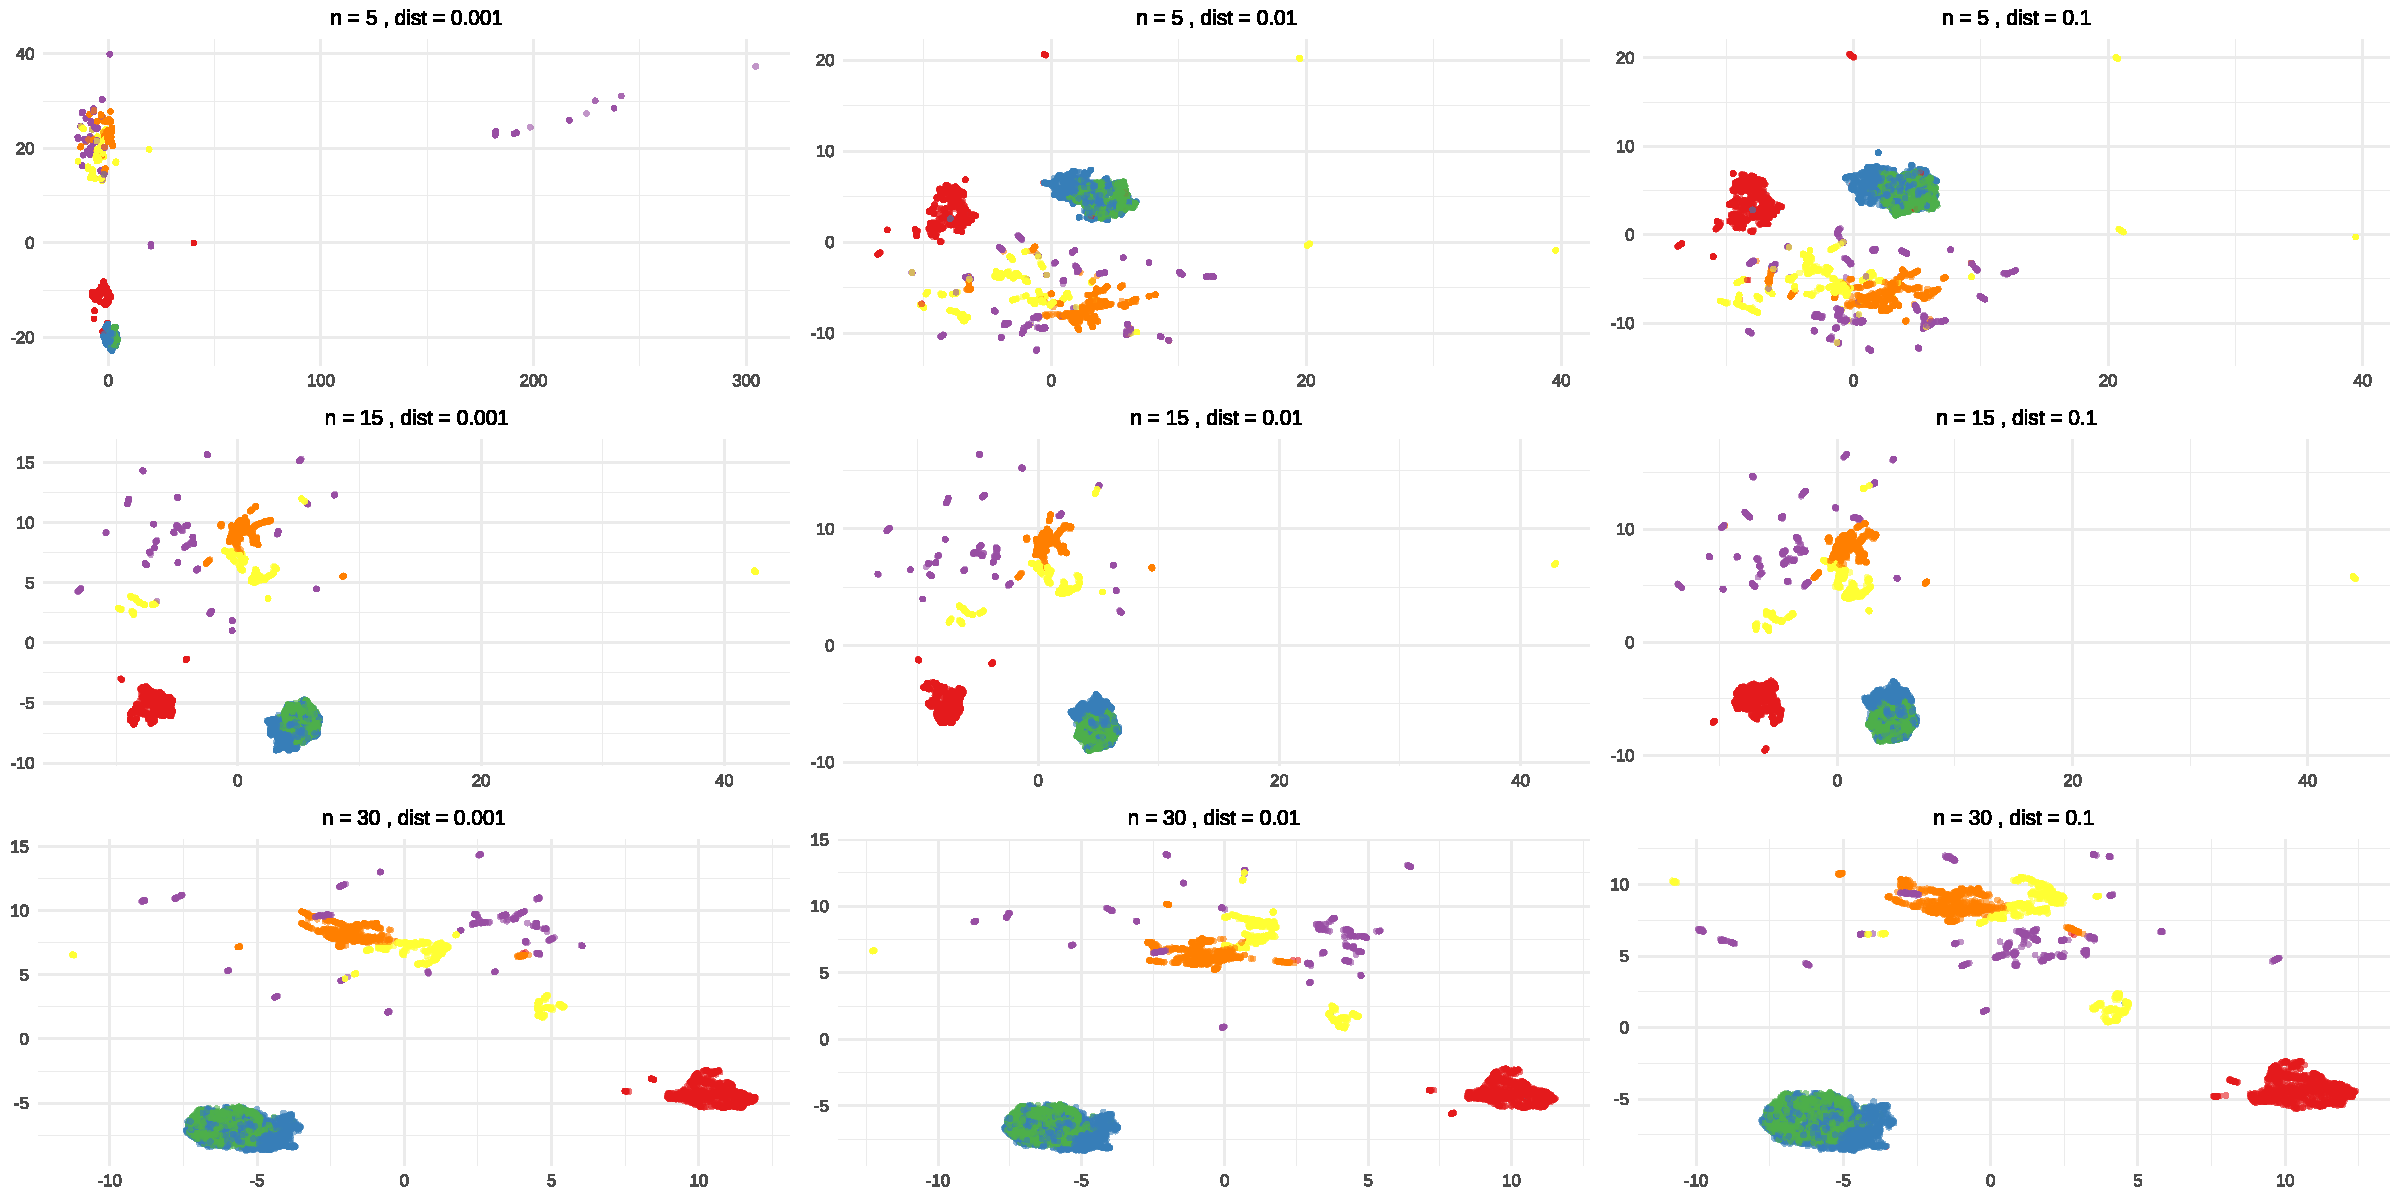
\includegraphics{report_files/figure-latex/unnamed-chunk-21-1.pdf}
\caption{trực quan hóa UMAP}
\end{figure}

Khi \textbf{n\_neighbors = 5} mạng lưới lân cận nhỏ, cấu trúc cục bộ
lỏng lẻo và thiếu kết nối giữa các cụm, các cụm co mạnh nhưng phân bố
không đồng đều. \textbf{n neighbors = 15} cấu trúc dữ liệu trở nên rõ
ràng hơn. Khi kết hợp với min dist = 0.01, các cụm đại diện cho các chức
năng khác nhau bắt đầu được hình thành rõ ràng và phân chia khá mạch
lạc, thể hiện sự phân cấp cao giữa các đối tượng, các cụm nhỏ như
sitting và lay ing bắt đầu được gom sát nhau. \textbf{n\_neighbors = 30}
thể hiện cấu trúc dữ liệu ổn định hơn. Dữ liệu được sắp xếp hợp lý, thấy
được sự ổn định trong phân cụm. Đặc biệt với min\_dist = 0.1, dữ liệu
dàn rộng hơn trong không gian nhúng, phù hợp cho việc phân tích tổng
thể.

Kết quả phân tích thấy được các siêu tham số n neighbors = 30 và min
dist = 0.1 tạo ra hình ảnh không gian nhúng chính xác và có sự phân biệt
tốt nhất giữa các hoạt động. Đây là cơ sở quan trọng giúp xác định cấu
hình tối ưu khi dùng UMAP như một bước tiền xử lý trong pipeline học
máy.

\begin{itemize}
\tightlist
\item
  Dựa vào kết phân tích hệ thống các siêu tham số trong kỹ thuật giảm
  chiều UMAP thì cấu hình n\_neighbors = 30 và min\_dist = 0.01 đã được
  xác định là một trong những cấu hình hiệu quả nhất để đảm bảo cấu trúc
  dữ liệu và phân tách các nhãn rõ ràng. Chúng em sẽ tiến hành minh họa
  kết quả giảm chiều dữ liệu cảm biến từ 561 đặc trưng về 2 chiều, áp
  dụng các cấu hinhg tối ưu nêu trên, mỗi điểm là đại diện cho một mẫu
  dữ liệu và được tô mày theo loại hoạt động được gán nhãn.
\end{itemize}

\begin{Shaded}
\begin{Highlighting}[]
\FunctionTok{library}\NormalTok{(umap)}
\FunctionTok{library}\NormalTok{(ggplot2)}

\NormalTok{config }\OtherTok{\textless{}{-}}\NormalTok{ umap.defaults}
\NormalTok{config}\SpecialCharTok{$}\NormalTok{n\_neighbors }\OtherTok{\textless{}{-}} \DecValTok{30}
\NormalTok{config}\SpecialCharTok{$}\NormalTok{min\_dist }\OtherTok{\textless{}{-}} \FloatTok{0.1}
\NormalTok{config}\SpecialCharTok{$}\NormalTok{n\_components }\OtherTok{\textless{}{-}} \DecValTok{2}

\NormalTok{umap\_result }\OtherTok{\textless{}{-}} \FunctionTok{umap}\NormalTok{(sensor\_data\_capped, }\AttributeTok{config =}\NormalTok{ config)}

\NormalTok{umap\_df }\OtherTok{\textless{}{-}} \FunctionTok{as.data.frame}\NormalTok{(umap\_result}\SpecialCharTok{$}\NormalTok{layout)}
\FunctionTok{colnames}\NormalTok{(umap\_df) }\OtherTok{\textless{}{-}} \FunctionTok{c}\NormalTok{(}\StringTok{"UMAP\_1"}\NormalTok{, }\StringTok{"UMAP\_2"}\NormalTok{)}
\NormalTok{umap\_df}\SpecialCharTok{$}\NormalTok{Activity }\OtherTok{\textless{}{-}}\NormalTok{ train}\SpecialCharTok{$}\NormalTok{Activity}

\FunctionTok{ggplot}\NormalTok{(umap\_df, }\FunctionTok{aes}\NormalTok{(}\AttributeTok{x =}\NormalTok{ UMAP\_1, }\AttributeTok{y =}\NormalTok{ UMAP\_2, }\AttributeTok{color =}\NormalTok{ Activity)) }\SpecialCharTok{+}
  \FunctionTok{geom\_point}\NormalTok{(}\AttributeTok{size =} \FloatTok{0.7}\NormalTok{, }\AttributeTok{alpha =} \FloatTok{0.6}\NormalTok{) }\SpecialCharTok{+}
  \FunctionTok{scale\_color\_brewer}\NormalTok{(}\AttributeTok{palette =} \StringTok{"Set1"}\NormalTok{) }\SpecialCharTok{+}
  \FunctionTok{theme\_minimal}\NormalTok{(}\AttributeTok{base\_size =} \DecValTok{14}\NormalTok{) }\SpecialCharTok{+}
  \FunctionTok{labs}\NormalTok{(}
    \AttributeTok{title =} \StringTok{"UMAP (n\_neighbors = 30, min\_dist = 0.01)"}\NormalTok{,}
    \AttributeTok{x =} \StringTok{"UMAP 1"}\NormalTok{, }\AttributeTok{y =} \StringTok{"UMAP 2"}
\NormalTok{  )}
\end{Highlighting}
\end{Shaded}

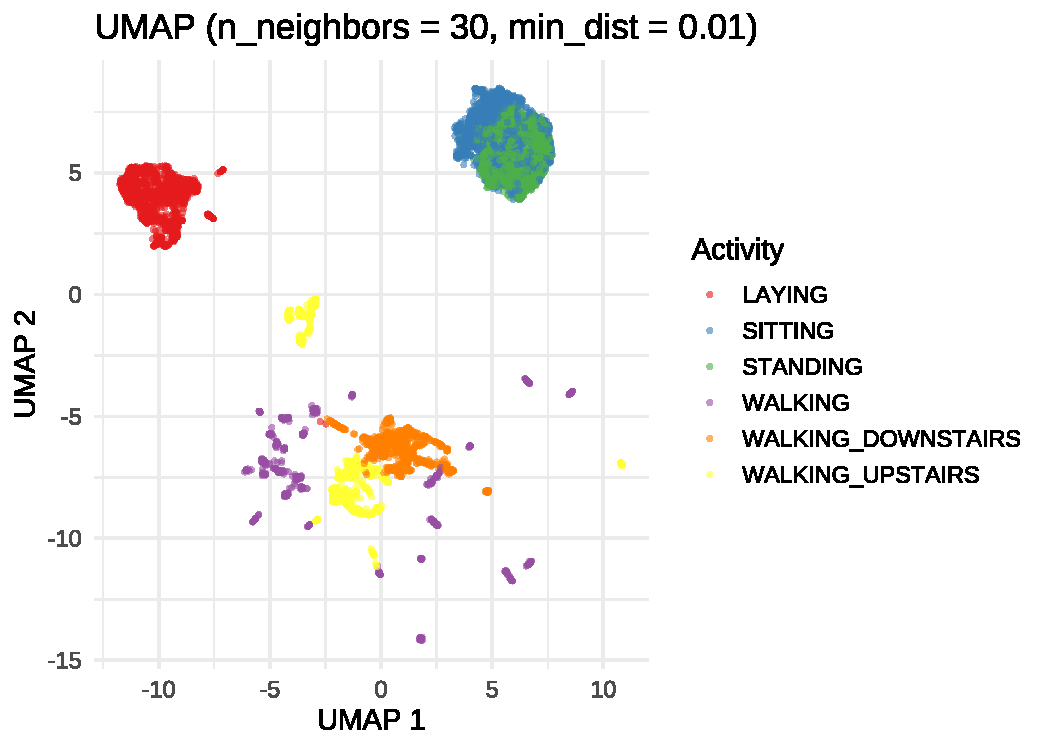
\includegraphics{report_files/figure-latex/unnamed-chunk-22-1.pdf} Các
hoạt động như LAYING, SITTING và STANDING tạo thành ba cụm rõ ràng, thấy
được tín hiệu cảm biến ở trong thái tĩnh có sự ổn định cao và dễ phân
biệt. Các hoạt động như WALKING, WALKING\_DOWNSTAIRS, WALKING\_UPSTAIRS
có xu hướng gần nhau hơn trong không gian 2 chiều, mặc dù vẫn tạo thành
các cụm riêng biệt, nhưng vẫn có vẻ chồng lấn, cho thấy được biến thiên
phức tạp của vận động trong thực tế. Thấy được sự tách biệt rõ ràng giữa
các nhóm động và tĩnh. Đây là bước tiền xử lý và kiểm định trực quan
quan trọng trước khi đưa dữ liệu vào các thuật toán học máy như Random
Forest, SVM, Logistic Regression và k-NN.

\subsection{Chuẩn bị dữ liệu cho mô hình học
máy}\label{chuux1ea9n-bux1ecb-dux1eef-liux1ec7u-cho-muxf4-huxecnh-hux1ecdc-muxe1y}

Sau khi hoàn thành các bước tiền xử lý, tập dữ liệu được chia thành hai
thành phần chính: ma trận đặc trưng đầu vào và nhãn đầu ra tương ứng.
Các biến định danh như subject và Activity được loại bỏ khỏi ma trận đặc
trưng, nhằm đảm bảo mô hình chỉ học từ các tín hiệu cảm biến mà không bị
ảnh hưởng bởi thông tin định danh.

\begin{Shaded}
\begin{Highlighting}[]
\NormalTok{X\_train }\OtherTok{\textless{}{-}}\NormalTok{ train\_capped[, }\SpecialCharTok{!}\NormalTok{(}\FunctionTok{names}\NormalTok{(train\_capped) }\SpecialCharTok{\%in\%} \FunctionTok{c}\NormalTok{(}\StringTok{"subject"}\NormalTok{, }\StringTok{"Activity"}\NormalTok{))]}
\NormalTok{y\_train }\OtherTok{\textless{}{-}}\NormalTok{ train\_capped}\SpecialCharTok{$}\NormalTok{Activity}

\NormalTok{X\_test }\OtherTok{\textless{}{-}}\NormalTok{ test\_capped[, }\SpecialCharTok{!}\NormalTok{(}\FunctionTok{names}\NormalTok{(test\_capped) }\SpecialCharTok{\%in\%} \FunctionTok{c}\NormalTok{(}\StringTok{"subject"}\NormalTok{, }\StringTok{"Activity"}\NormalTok{))]}
\NormalTok{y\_test }\OtherTok{\textless{}{-}}\NormalTok{ test\_capped}\SpecialCharTok{$}\NormalTok{Activity}

\FunctionTok{dim}\NormalTok{(X\_train)}
\end{Highlighting}
\end{Shaded}

\begin{verbatim}
## [1] 7352  561
\end{verbatim}

\begin{Shaded}
\begin{Highlighting}[]
\FunctionTok{length}\NormalTok{(y\_train)}
\end{Highlighting}
\end{Shaded}

\begin{verbatim}
## [1] 7352
\end{verbatim}

\begin{Shaded}
\begin{Highlighting}[]
\FunctionTok{dim}\NormalTok{(X\_test)}
\end{Highlighting}
\end{Shaded}

\begin{verbatim}
## [1] 2947  561
\end{verbatim}

\begin{Shaded}
\begin{Highlighting}[]
\FunctionTok{length}\NormalTok{(y\_test)}
\end{Highlighting}
\end{Shaded}

\begin{verbatim}
## [1] 2947
\end{verbatim}

\subsection{xây dựng hàm đánh giá tổng quá mô hình học
máy}\label{xuxe2y-dux1ef1ng-huxe0m-ux111uxe1nh-giuxe1-tux1ed5ng-quuxe1-muxf4-huxecnh-hux1ecdc-muxe1y}

Để đảm bảo sự thống nhất và tái sử dụng trong việc đào tạo và đánh giá
các mô hình học máy, một hàm tổng quát có tên
train\_and\_evaluate\_model đã được thiết lập.Hàm thực hiện quy trình
huấn luyện, dự đoán, đánh giá và trực quan hóa kết quả của một mô hình
phân loại với cấu trúc linh hoạt, cho phép sử dụng nhiều thuật toán khác
nhau như Random Forest, SVM, Logistic Regression, hoặc k-NN.

\begin{Shaded}
\begin{Highlighting}[]
\NormalTok{train\_and\_evaluate\_model }\OtherTok{\textless{}{-}} \ControlFlowTok{function}\NormalTok{(}
\NormalTok{  model\_name,}
\NormalTok{  X\_train, y\_train, X\_test, y\_test,}
\NormalTok{  class\_labels,}
  \AttributeTok{tuneGrid =} \ConstantTok{NULL}\NormalTok{,}
  \AttributeTok{k\_folds =} \DecValTok{5}
\NormalTok{) \{}
  \ControlFlowTok{if}\NormalTok{ (}\SpecialCharTok{!}\FunctionTok{require}\NormalTok{(caret)) }\FunctionTok{install.packages}\NormalTok{(}\StringTok{"caret"}\NormalTok{, }\AttributeTok{quiet =} \ConstantTok{TRUE}\NormalTok{)}
  \ControlFlowTok{if}\NormalTok{ (}\SpecialCharTok{!}\FunctionTok{require}\NormalTok{(ggplot2)) }\FunctionTok{install.packages}\NormalTok{(}\StringTok{"ggplot2"}\NormalTok{, }\AttributeTok{quiet =} \ConstantTok{TRUE}\NormalTok{)}

  \FunctionTok{library}\NormalTok{(caret)}
  \FunctionTok{library}\NormalTok{(ggplot2)}

\NormalTok{  y\_train }\OtherTok{\textless{}{-}} \FunctionTok{as.factor}\NormalTok{(y\_train)}
\NormalTok{  y\_test }\OtherTok{\textless{}{-}} \FunctionTok{as.factor}\NormalTok{(y\_test)}

\NormalTok{  ctrl }\OtherTok{\textless{}{-}} \FunctionTok{trainControl}\NormalTok{(}\AttributeTok{method =} \StringTok{"cv"}\NormalTok{, }\AttributeTok{number =}\NormalTok{ k\_folds)}

  \FunctionTok{set.seed}\NormalTok{(}\DecValTok{123}\NormalTok{)}
\NormalTok{  model\_fit }\OtherTok{\textless{}{-}} \FunctionTok{train}\NormalTok{(}
    \AttributeTok{x =}\NormalTok{ X\_train,}
    \AttributeTok{y =}\NormalTok{ y\_train,}
    \AttributeTok{method =}\NormalTok{ model\_name,}
    \AttributeTok{trControl =}\NormalTok{ ctrl,}
    \AttributeTok{tuneGrid =}\NormalTok{ tuneGrid}
\NormalTok{  )}

\NormalTok{  y\_pred }\OtherTok{\textless{}{-}} \FunctionTok{predict}\NormalTok{(model\_fit, X\_test)}

  \CommentTok{\# Accuracy}
\NormalTok{  accuracy }\OtherTok{\textless{}{-}} \FunctionTok{mean}\NormalTok{(y\_pred }\SpecialCharTok{==}\NormalTok{ y\_test)}
  \FunctionTok{cat}\NormalTok{(}\StringTok{"{-}{-}{-}{-}{-}{-}{-}{-}{-}{-}{-}{-}{-}{-}{-}{-}{-}{-}{-}{-}{-}}\SpecialCharTok{\textbackslash{}n}\StringTok{"}\NormalTok{)}
  \FunctionTok{cat}\NormalTok{(}\StringTok{"|      Accuracy      |}\SpecialCharTok{\textbackslash{}n}\StringTok{"}\NormalTok{)}
  \FunctionTok{cat}\NormalTok{(}\StringTok{"{-}{-}{-}{-}{-}{-}{-}{-}{-}{-}{-}{-}{-}{-}{-}{-}{-}{-}{-}{-}{-}}\SpecialCharTok{\textbackslash{}n}\StringTok{"}\NormalTok{)}
  \FunctionTok{cat}\NormalTok{(}\FunctionTok{sprintf}\NormalTok{(}\StringTok{"}\SpecialCharTok{\textbackslash{}n}\StringTok{    \%.4f}\SpecialCharTok{\textbackslash{}n\textbackslash{}n}\StringTok{"}\NormalTok{, accuracy))}

  \CommentTok{\# Confusion matrix}
\NormalTok{  cm }\OtherTok{\textless{}{-}} \FunctionTok{table}\NormalTok{(}\AttributeTok{Predicted =}\NormalTok{ y\_pred, }\AttributeTok{Actual =}\NormalTok{ y\_test)}
  \FunctionTok{cat}\NormalTok{(}\StringTok{"{-}{-}{-}{-}{-}{-}{-}{-}{-}{-}{-}{-}{-}{-}{-}{-}{-}{-}{-}{-}}\SpecialCharTok{\textbackslash{}n}\StringTok{"}\NormalTok{)}
  \FunctionTok{cat}\NormalTok{(}\StringTok{"| Confusion Matrix |}\SpecialCharTok{\textbackslash{}n}\StringTok{"}\NormalTok{)}
  \FunctionTok{cat}\NormalTok{(}\StringTok{"{-}{-}{-}{-}{-}{-}{-}{-}{-}{-}{-}{-}{-}{-}{-}{-}{-}{-}{-}{-}}\SpecialCharTok{\textbackslash{}n}\StringTok{"}\NormalTok{)}
  \FunctionTok{print}\NormalTok{(cm)}

  \CommentTok{\# Plot confusion matrix}
\NormalTok{  cm\_df }\OtherTok{\textless{}{-}} \FunctionTok{as.data.frame}\NormalTok{(cm)}
  \FunctionTok{colnames}\NormalTok{(cm\_df) }\OtherTok{\textless{}{-}} \FunctionTok{c}\NormalTok{(}\StringTok{"Predicted"}\NormalTok{, }\StringTok{"Actual"}\NormalTok{, }\StringTok{"Freq"}\NormalTok{)}

  \FunctionTok{ggplot}\NormalTok{(}\AttributeTok{data =}\NormalTok{ cm\_df, }\FunctionTok{aes}\NormalTok{(}\AttributeTok{x =}\NormalTok{ Actual, }\AttributeTok{y =}\NormalTok{ Predicted, }\AttributeTok{fill =}\NormalTok{ Freq)) }\SpecialCharTok{+}
    \FunctionTok{geom\_tile}\NormalTok{(}\AttributeTok{color =} \StringTok{"white"}\NormalTok{) }\SpecialCharTok{+}
    \FunctionTok{geom\_text}\NormalTok{(}\FunctionTok{aes}\NormalTok{(}\AttributeTok{label =}\NormalTok{ Freq), }\AttributeTok{color =} \StringTok{"black"}\NormalTok{, }\AttributeTok{size =} \DecValTok{5}\NormalTok{) }\SpecialCharTok{+}
    \FunctionTok{scale\_fill\_gradient}\NormalTok{(}\AttributeTok{low =} \StringTok{"white"}\NormalTok{, }\AttributeTok{high =} \StringTok{"darkgreen"}\NormalTok{) }\SpecialCharTok{+}
    \FunctionTok{labs}\NormalTok{(}\AttributeTok{title =} \StringTok{"Confusion Matrix"}\NormalTok{, }\AttributeTok{x =} \StringTok{"True Label"}\NormalTok{, }\AttributeTok{y =} \StringTok{"Predicted Label"}\NormalTok{) }\SpecialCharTok{+}
    \FunctionTok{theme\_minimal}\NormalTok{() }\SpecialCharTok{+}
    \FunctionTok{theme}\NormalTok{(}\AttributeTok{axis.text.x =} \FunctionTok{element\_text}\NormalTok{(}\AttributeTok{angle =} \DecValTok{45}\NormalTok{, }\AttributeTok{hjust =} \DecValTok{1}\NormalTok{))}

  \CommentTok{\# Classification report}
  \FunctionTok{cat}\NormalTok{(}\StringTok{"{-}{-}{-}{-}{-}{-}{-}{-}{-}{-}{-}{-}{-}{-}{-}{-}{-}{-}{-}{-}{-}{-}{-}{-}{-}}\SpecialCharTok{\textbackslash{}n}\StringTok{"}\NormalTok{)}
  \FunctionTok{cat}\NormalTok{(}\StringTok{"| Classification Report |}\SpecialCharTok{\textbackslash{}n}\StringTok{"}\NormalTok{)}
  \FunctionTok{cat}\NormalTok{(}\StringTok{"{-}{-}{-}{-}{-}{-}{-}{-}{-}{-}{-}{-}{-}{-}{-}{-}{-}{-}{-}{-}{-}{-}{-}{-}{-}}\SpecialCharTok{\textbackslash{}n}\StringTok{"}\NormalTok{)}
  \FunctionTok{print}\NormalTok{(}\FunctionTok{confusionMatrix}\NormalTok{(y\_pred, y\_test)}\SpecialCharTok{$}\NormalTok{byClass)}

  \FunctionTok{cat}\NormalTok{(}\StringTok{\textquotesingle{}{-}{-}{-}{-}{-}{-}{-}{-}{-}{-}{-}{-}{-}{-}{-}{-}{-}{-}{-}{-}{-}{-}{-}{-}{-}{-}}\SpecialCharTok{\textbackslash{}n}\StringTok{\textquotesingle{}}\NormalTok{)}
  \FunctionTok{cat}\NormalTok{(}\StringTok{\textquotesingle{}|     Best Parameters     |}\SpecialCharTok{\textbackslash{}n}\StringTok{\textquotesingle{}}\NormalTok{)}
  \FunctionTok{cat}\NormalTok{(}\StringTok{\textquotesingle{}{-}{-}{-}{-}{-}{-}{-}{-}{-}{-}{-}{-}{-}{-}{-}{-}{-}{-}{-}{-}{-}{-}{-}{-}{-}{-}}\SpecialCharTok{\textbackslash{}n}\StringTok{\textquotesingle{}}\NormalTok{)}
  \FunctionTok{print}\NormalTok{(model\_fit}\SpecialCharTok{$}\NormalTok{bestTune)}

  \FunctionTok{cat}\NormalTok{(}\StringTok{\textquotesingle{}{-}{-}{-}{-}{-}{-}{-}{-}{-}{-}{-}{-}{-}{-}{-}{-}{-}{-}{-}{-}{-}{-}{-}{-}{-}{-}}\SpecialCharTok{\textbackslash{}n}\StringTok{\textquotesingle{}}\NormalTok{)}
  \FunctionTok{cat}\NormalTok{(}\StringTok{\textquotesingle{}|      Best Accuracy      |}\SpecialCharTok{\textbackslash{}n}\StringTok{\textquotesingle{}}\NormalTok{)}
  \FunctionTok{cat}\NormalTok{(}\StringTok{\textquotesingle{}{-}{-}{-}{-}{-}{-}{-}{-}{-}{-}{-}{-}{-}{-}{-}{-}{-}{-}{-}{-}{-}{-}{-}{-}{-}{-}}\SpecialCharTok{\textbackslash{}n}\StringTok{\textquotesingle{}}\NormalTok{)}
  \FunctionTok{print}\NormalTok{(}\FunctionTok{max}\NormalTok{(model\_fit}\SpecialCharTok{$}\NormalTok{results}\SpecialCharTok{$}\NormalTok{Accuracy))}

  \FunctionTok{return}\NormalTok{(}\FunctionTok{list}\NormalTok{(}
    \AttributeTok{model =}\NormalTok{ model\_fit,}
    \AttributeTok{accuracy =}\NormalTok{ accuracy,}
    \AttributeTok{confusion\_matrix =}\NormalTok{ cm,}
    \AttributeTok{prediction =}\NormalTok{ y\_pred}
\NormalTok{  ))}
\NormalTok{\}}
\end{Highlighting}
\end{Shaded}

\begin{Shaded}
\begin{Highlighting}[]
\NormalTok{grid\_logistic }\OtherTok{\textless{}{-}} \FunctionTok{expand.grid}\NormalTok{(}
  \AttributeTok{alpha =} \FunctionTok{c}\NormalTok{(}\DecValTok{0}\NormalTok{, }\DecValTok{1}\NormalTok{),}
  \AttributeTok{lambda =} \DecValTok{1} \SpecialCharTok{/} \FunctionTok{c}\NormalTok{(}\FloatTok{0.01}\NormalTok{, }\FloatTok{0.1}\NormalTok{, }\DecValTok{1}\NormalTok{, }\DecValTok{10}\NormalTok{, }\DecValTok{20}\NormalTok{, }\DecValTok{30}\NormalTok{)}
\NormalTok{)}

\NormalTok{results\_log }\OtherTok{\textless{}{-}} \FunctionTok{train\_and\_evaluate\_model}\NormalTok{(}
  \AttributeTok{model\_name =} \StringTok{"glmnet"}\NormalTok{,}
  \AttributeTok{X\_train =}\NormalTok{ X\_train, }\AttributeTok{y\_train =}\NormalTok{ y\_train,}
  \AttributeTok{X\_test =}\NormalTok{ X\_test, }\AttributeTok{y\_test =}\NormalTok{ y\_test,}
  \AttributeTok{class\_labels =}\NormalTok{ labels,}
  \AttributeTok{tuneGrid =}\NormalTok{ grid\_logistic,}
  \AttributeTok{k\_folds =} \DecValTok{5}
\NormalTok{)}
\end{Highlighting}
\end{Shaded}

\begin{verbatim}
## Loading required package: caret
\end{verbatim}

\begin{verbatim}
## Loading required package: lattice
\end{verbatim}

\begin{verbatim}
## ---------------------
## |      Accuracy      |
## ---------------------
## 
##     0.9488
## 
## --------------------
## | Confusion Matrix |
## --------------------
##                     Actual
## Predicted            LAYING SITTING STANDING WALKING WALKING_DOWNSTAIRS
##   LAYING                537       0        0       0                  0
##   SITTING                 0     431       30       0                  0
##   STANDING                0      57      502       0                  0
##   WALKING                 0       0        0     493                 10
##   WALKING_DOWNSTAIRS      0       0        0       3                387
##   WALKING_UPSTAIRS        0       3        0       0                 23
##                     Actual
## Predicted            WALKING_UPSTAIRS
##   LAYING                            0
##   SITTING                           0
##   STANDING                          1
##   WALKING                          22
##   WALKING_DOWNSTAIRS                2
##   WALKING_UPSTAIRS                446
## -------------------------
## | Classification Report |
## -------------------------
##                           Sensitivity Specificity Pos Pred Value Neg Pred Value
## Class: LAYING               1.0000000   1.0000000      1.0000000      1.0000000
## Class: SITTING              0.8778004   0.9877850      0.9349241      0.9758648
## Class: STANDING             0.9436090   0.9759834      0.8964286      0.9874319
## Class: WALKING              0.9939516   0.9869441      0.9390476      0.9987614
## Class: WALKING_DOWNSTAIRS   0.9214286   0.9980214      0.9872449      0.9870841
## Class: WALKING_UPSTAIRS     0.9469214   0.9894992      0.9449153      0.9898990
##                           Precision    Recall        F1 Prevalence
## Class: LAYING             1.0000000 1.0000000 1.0000000  0.1822192
## Class: SITTING            0.9349241 0.8778004 0.9054622  0.1666101
## Class: STANDING           0.8964286 0.9436090 0.9194139  0.1805226
## Class: WALKING            0.9390476 0.9939516 0.9657199  0.1683068
## Class: WALKING_DOWNSTAIRS 0.9872449 0.9214286 0.9532020  0.1425178
## Class: WALKING_UPSTAIRS   0.9449153 0.9469214 0.9459173  0.1598235
##                           Detection Rate Detection Prevalence Balanced Accuracy
## Class: LAYING                  0.1822192            0.1822192         1.0000000
## Class: SITTING                 0.1462504            0.1564303         0.9327927
## Class: STANDING                0.1703427            0.1900238         0.9597962
## Class: WALKING                 0.1672888            0.1781473         0.9904479
## Class: WALKING_DOWNSTAIRS      0.1313200            0.1330166         0.9597250
## Class: WALKING_UPSTAIRS        0.1513403            0.1601629         0.9682103
## --------------------------
## |     Best Parameters     |
## --------------------------
##   alpha     lambda
## 1     0 0.03333333
## --------------------------
## |      Best Accuracy      |
## --------------------------
## [1] 0.9688516
\end{verbatim}

\begin{Shaded}
\begin{Highlighting}[]
\NormalTok{grid\_linear\_svc }\OtherTok{\textless{}{-}} \FunctionTok{expand.grid}\NormalTok{(}\AttributeTok{C =} \FunctionTok{c}\NormalTok{(}\FloatTok{0.125}\NormalTok{, }\FloatTok{0.5}\NormalTok{, }\DecValTok{1}\NormalTok{, }\DecValTok{2}\NormalTok{, }\DecValTok{8}\NormalTok{, }\DecValTok{16}\NormalTok{))}

\NormalTok{results\_svc }\OtherTok{\textless{}{-}} \FunctionTok{train\_and\_evaluate\_model}\NormalTok{(}
  \AttributeTok{model\_name =} \StringTok{"svmLinear"}\NormalTok{,}
  \AttributeTok{X\_train =}\NormalTok{ X\_train, }\AttributeTok{y\_train =}\NormalTok{ y\_train,}
  \AttributeTok{X\_test =}\NormalTok{ X\_test, }\AttributeTok{y\_test =}\NormalTok{ y\_test,}
  \AttributeTok{class\_labels =}\NormalTok{ labels,}
  \AttributeTok{tuneGrid =}\NormalTok{ grid\_linear\_svc,}
  \AttributeTok{k\_folds =} \DecValTok{5}
\NormalTok{)}
\end{Highlighting}
\end{Shaded}

\begin{verbatim}
## ---------------------
## |      Accuracy      |
## ---------------------
## 
##     0.9606
## 
## --------------------
## | Confusion Matrix |
## --------------------
##                     Actual
## Predicted            LAYING SITTING STANDING WALKING WALKING_DOWNSTAIRS
##   LAYING                537       0        0       0                  0
##   SITTING                 0     436       16       0                  0
##   STANDING                0      53      516       0                  0
##   WALKING                 0       0        0     493                  5
##   WALKING_DOWNSTAIRS      0       0        0       2                399
##   WALKING_UPSTAIRS        0       2        0       1                 16
##                     Actual
## Predicted            WALKING_UPSTAIRS
##   LAYING                            0
##   SITTING                           0
##   STANDING                          0
##   WALKING                          16
##   WALKING_DOWNSTAIRS                5
##   WALKING_UPSTAIRS                450
## -------------------------
## | Classification Report |
## -------------------------
##                           Sensitivity Specificity Pos Pred Value Neg Pred Value
## Class: LAYING               1.0000000   1.0000000      1.0000000      1.0000000
## Class: SITTING              0.8879837   0.9934853      0.9646018      0.9779559
## Class: STANDING             0.9699248   0.9780538      0.9068541      0.9932717
## Class: WALKING              0.9939516   0.9914321      0.9591440      0.9987670
## Class: WALKING_DOWNSTAIRS   0.9500000   0.9972299      0.9827586      0.9917355
## Class: WALKING_UPSTAIRS     0.9554140   0.9923263      0.9594883      0.9915254
##                           Precision    Recall        F1 Prevalence
## Class: LAYING             1.0000000 1.0000000 1.0000000  0.1822192
## Class: SITTING            0.9646018 0.8879837 0.9247084  0.1666101
## Class: STANDING           0.9068541 0.9699248 0.9373297  0.1805226
## Class: WALKING            0.9591440 0.9939516 0.9762376  0.1683068
## Class: WALKING_DOWNSTAIRS 0.9827586 0.9500000 0.9661017  0.1425178
## Class: WALKING_UPSTAIRS   0.9594883 0.9554140 0.9574468  0.1598235
##                           Detection Rate Detection Prevalence Balanced Accuracy
## Class: LAYING                  0.1822192            0.1822192         1.0000000
## Class: SITTING                 0.1479471            0.1533763         0.9407345
## Class: STANDING                0.1750933            0.1930777         0.9739893
## Class: WALKING                 0.1672888            0.1744147         0.9926918
## Class: WALKING_DOWNSTAIRS      0.1353919            0.1377672         0.9736150
## Class: WALKING_UPSTAIRS        0.1526977            0.1591449         0.9738702
## --------------------------
## |     Best Parameters     |
## --------------------------
##       C
## 1 0.125
## --------------------------
## |      Best Accuracy      |
## --------------------------
## [1] 0.9844929
\end{verbatim}

\begin{Shaded}
\begin{Highlighting}[]
\NormalTok{grid\_dt }\OtherTok{\textless{}{-}} \FunctionTok{expand.grid}\NormalTok{(}\AttributeTok{maxdepth =} \FunctionTok{seq}\NormalTok{(}\DecValTok{3}\NormalTok{, }\DecValTok{9}\NormalTok{, }\AttributeTok{by =} \DecValTok{2}\NormalTok{))}

\NormalTok{results\_dt }\OtherTok{\textless{}{-}} \FunctionTok{train\_and\_evaluate\_model}\NormalTok{(}
  \AttributeTok{model\_name =} \StringTok{"rpart2"}\NormalTok{,}
  \AttributeTok{X\_train =}\NormalTok{ X\_train,}
  \AttributeTok{y\_train =}\NormalTok{ y\_train,}
  \AttributeTok{X\_test =}\NormalTok{ X\_test,}
  \AttributeTok{y\_test =}\NormalTok{ y\_test,}
  \AttributeTok{class\_labels =}\NormalTok{ labels,}
  \AttributeTok{tuneGrid =}\NormalTok{ grid\_dt,}
  \AttributeTok{k\_folds =} \DecValTok{5}
\NormalTok{)}
\end{Highlighting}
\end{Shaded}

\begin{verbatim}
## ---------------------
## |      Accuracy      |
## ---------------------
## 
##     0.8402
## 
## --------------------
## | Confusion Matrix |
## --------------------
##                     Actual
## Predicted            LAYING SITTING STANDING WALKING WALKING_DOWNSTAIRS
##   LAYING                537       0        0       0                  0
##   SITTING                 0     400      107       0                  0
##   STANDING                0      91      425       0                  0
##   WALKING                 0       0        0     430                 40
##   WALKING_DOWNSTAIRS      0       0        0      11                282
##   WALKING_UPSTAIRS        0       0        0      55                 98
##                     Actual
## Predicted            WALKING_UPSTAIRS
##   LAYING                            0
##   SITTING                           0
##   STANDING                          0
##   WALKING                          61
##   WALKING_DOWNSTAIRS                8
##   WALKING_UPSTAIRS                402
## -------------------------
## | Classification Report |
## -------------------------
##                           Sensitivity Specificity Pos Pred Value Neg Pred Value
## Class: LAYING               1.0000000   1.0000000      1.0000000      1.0000000
## Class: SITTING              0.8146640   0.9564332      0.7889546      0.9627049
## Class: STANDING             0.7988722   0.9623188      0.8236434      0.9559852
## Class: WALKING              0.8669355   0.9587923      0.8097928      0.9726821
## Class: WALKING_DOWNSTAIRS   0.6714286   0.9924812      0.9368771      0.9478458
## Class: WALKING_UPSTAIRS     0.8535032   0.9382068      0.7243243      0.9711538
##                           Precision    Recall        F1 Prevalence
## Class: LAYING             1.0000000 1.0000000 1.0000000  0.1822192
## Class: SITTING            0.7889546 0.8146640 0.8016032  0.1666101
## Class: STANDING           0.8236434 0.7988722 0.8110687  0.1805226
## Class: WALKING            0.8097928 0.8669355 0.8373905  0.1683068
## Class: WALKING_DOWNSTAIRS 0.9368771 0.6714286 0.7822469  0.1425178
## Class: WALKING_UPSTAIRS   0.7243243 0.8535032 0.7836257  0.1598235
##                           Detection Rate Detection Prevalence Balanced Accuracy
## Class: LAYING                 0.18221921            0.1822192         1.0000000
## Class: SITTING                0.13573125            0.1720394         0.8855486
## Class: STANDING               0.14421446            0.1750933         0.8805955
## Class: WALKING                0.14591110            0.1801832         0.9128639
## Class: WALKING_DOWNSTAIRS     0.09569053            0.1021378         0.8319549
## Class: WALKING_UPSTAIRS       0.13640991            0.1883271         0.8958550
## --------------------------
## |     Best Parameters     |
## --------------------------
##   maxdepth
## 3        7
## --------------------------
## |      Best Accuracy      |
## --------------------------
## [1] 0.8860176
\end{verbatim}

\begin{Shaded}
\begin{Highlighting}[]
\FunctionTok{library}\NormalTok{(randomForest)}
\end{Highlighting}
\end{Shaded}

\begin{verbatim}
## randomForest 4.7-1.2
\end{verbatim}

\begin{verbatim}
## Type rfNews() to see new features/changes/bug fixes.
\end{verbatim}

\begin{verbatim}
## 
## Attaching package: 'randomForest'
\end{verbatim}

\begin{verbatim}
## The following object is masked from 'package:gridExtra':
## 
##     combine
\end{verbatim}

\begin{verbatim}
## The following object is masked from 'package:dplyr':
## 
##     combine
\end{verbatim}

\begin{verbatim}
## The following object is masked from 'package:ggplot2':
## 
##     margin
\end{verbatim}

\begin{Shaded}
\begin{Highlighting}[]
\NormalTok{grid\_rf }\OtherTok{\textless{}{-}} \FunctionTok{expand.grid}\NormalTok{(}\AttributeTok{mtry =} \FunctionTok{c}\NormalTok{(}\DecValTok{16}\NormalTok{, }\DecValTok{20}\NormalTok{, }\DecValTok{24}\NormalTok{, }\DecValTok{28}\NormalTok{, }\DecValTok{32}\NormalTok{))}
\NormalTok{results\_rf }\OtherTok{\textless{}{-}} \FunctionTok{train\_and\_evaluate\_model}\NormalTok{(}
  \AttributeTok{model\_name =} \StringTok{"rf"}\NormalTok{,}
  \AttributeTok{X\_train =}\NormalTok{ X\_train,}
  \AttributeTok{y\_train =}\NormalTok{ y\_train,}
  \AttributeTok{X\_test =}\NormalTok{ X\_test,}
  \AttributeTok{y\_test =}\NormalTok{ y\_test,}
  \AttributeTok{class\_labels =}\NormalTok{ labels,}
  \AttributeTok{tuneGrid =}\NormalTok{ grid\_rf,}
  \AttributeTok{k\_folds =} \DecValTok{5}
\NormalTok{)}
\end{Highlighting}
\end{Shaded}

\begin{verbatim}
## ---------------------
## |      Accuracy      |
## ---------------------
## 
##     0.9355
## 
## --------------------
## | Confusion Matrix |
## --------------------
##                     Actual
## Predicted            LAYING SITTING STANDING WALKING WALKING_DOWNSTAIRS
##   LAYING                537       0        0       0                  0
##   SITTING                 0     448       29       0                  0
##   STANDING                0      43      503       0                  0
##   WALKING                 0       0        0     480                 19
##   WALKING_DOWNSTAIRS      0       0        0       8                354
##   WALKING_UPSTAIRS        0       0        0       8                 47
##                     Actual
## Predicted            WALKING_UPSTAIRS
##   LAYING                            0
##   SITTING                           0
##   STANDING                          0
##   WALKING                          30
##   WALKING_DOWNSTAIRS                6
##   WALKING_UPSTAIRS                435
## -------------------------
## | Classification Report |
## -------------------------
##                           Sensitivity Specificity Pos Pred Value Neg Pred Value
## Class: LAYING               1.0000000   1.0000000      1.0000000      1.0000000
## Class: SITTING              0.9124236   0.9881922      0.9392034      0.9825911
## Class: STANDING             0.9454887   0.9821946      0.9212454      0.9879217
## Class: WALKING              0.9677419   0.9800082      0.9073724      0.9933830
## Class: WALKING_DOWNSTAIRS   0.8428571   0.9944598      0.9619565      0.9744087
## Class: WALKING_UPSTAIRS     0.9235669   0.9777868      0.8877551      0.9853480
##                           Precision    Recall        F1 Prevalence
## Class: LAYING             1.0000000 1.0000000 1.0000000  0.1822192
## Class: SITTING            0.9392034 0.9124236 0.9256198  0.1666101
## Class: STANDING           0.9212454 0.9454887 0.9332096  0.1805226
## Class: WALKING            0.9073724 0.9677419 0.9365854  0.1683068
## Class: WALKING_DOWNSTAIRS 0.9619565 0.8428571 0.8984772  0.1425178
## Class: WALKING_UPSTAIRS   0.8877551 0.9235669 0.9053070  0.1598235
##                           Detection Rate Detection Prevalence Balanced Accuracy
## Class: LAYING                  0.1822192            0.1822192         1.0000000
## Class: SITTING                 0.1520190            0.1618595         0.9503079
## Class: STANDING                0.1706820            0.1852732         0.9638417
## Class: WALKING                 0.1628775            0.1795046         0.9738750
## Class: WALKING_DOWNSTAIRS      0.1201222            0.1248728         0.9186585
## Class: WALKING_UPSTAIRS        0.1476077            0.1662708         0.9506768
## --------------------------
## |     Best Parameters     |
## --------------------------
##   mtry
## 1   16
## --------------------------
## |      Best Accuracy      |
## --------------------------
## [1] 0.9829978
\end{verbatim}

\begin{Shaded}
\begin{Highlighting}[]
\NormalTok{grid\_knn }\OtherTok{\textless{}{-}} \FunctionTok{expand.grid}\NormalTok{(}\AttributeTok{k =} \FunctionTok{seq}\NormalTok{(}\DecValTok{1}\NormalTok{, }\DecValTok{30}\NormalTok{, }\AttributeTok{by =} \DecValTok{2}\NormalTok{))  }

\NormalTok{results\_knn }\OtherTok{\textless{}{-}} \FunctionTok{train\_and\_evaluate\_model}\NormalTok{(}
  \AttributeTok{model\_name =} \StringTok{"knn"}\NormalTok{,}
  \AttributeTok{X\_train =}\NormalTok{ X\_train, }
  \AttributeTok{y\_train =}\NormalTok{ y\_train,}
  \AttributeTok{X\_test =}\NormalTok{ X\_test, }
  \AttributeTok{y\_test =}\NormalTok{ y\_test,}
  \AttributeTok{class\_labels =}\NormalTok{ labels,}
  \AttributeTok{tuneGrid =}\NormalTok{ grid\_knn,}
  \AttributeTok{k\_folds =} \DecValTok{5}
\NormalTok{)}
\end{Highlighting}
\end{Shaded}

\begin{verbatim}
## ---------------------
## |      Accuracy      |
## ---------------------
## 
##     0.8799
## 
## --------------------
## | Confusion Matrix |
## --------------------
##                     Actual
## Predicted            LAYING SITTING STANDING WALKING WALKING_DOWNSTAIRS
##   LAYING                535       1        0       0                  0
##   SITTING                 2     393       80       0                  0
##   STANDING                0      96      452       0                  0
##   WALKING                 0       0        0     472                 53
##   WALKING_DOWNSTAIRS      0       0        0      13                317
##   WALKING_UPSTAIRS        0       1        0      11                 50
##                     Actual
## Predicted            WALKING_UPSTAIRS
##   LAYING                            0
##   SITTING                           0
##   STANDING                          0
##   WALKING                          29
##   WALKING_DOWNSTAIRS               18
##   WALKING_UPSTAIRS                424
## -------------------------
## | Classification Report |
## -------------------------
##                           Sensitivity Specificity Pos Pred Value Neg Pred Value
## Class: LAYING               0.9962756   0.9995851      0.9981343      0.9991705
## Class: SITTING              0.8004073   0.9666124      0.8273684      0.9603560
## Class: STANDING             0.8496241   0.9602484      0.8248175      0.9666528
## Class: WALKING              0.9516129   0.9665443      0.8519856      0.9899707
## Class: WALKING_DOWNSTAIRS   0.7547619   0.9877325      0.9109195      0.9603694
## Class: WALKING_UPSTAIRS     0.9002123   0.9749596      0.8724280      0.9809021
##                           Precision    Recall        F1 Prevalence
## Class: LAYING             0.9981343 0.9962756 0.9972041  0.1822192
## Class: SITTING            0.8273684 0.8004073 0.8136646  0.1666101
## Class: STANDING           0.8248175 0.8496241 0.8370370  0.1805226
## Class: WALKING            0.8519856 0.9516129 0.8990476  0.1683068
## Class: WALKING_DOWNSTAIRS 0.9109195 0.7547619 0.8255208  0.1425178
## Class: WALKING_UPSTAIRS   0.8724280 0.9002123 0.8861024  0.1598235
##                           Detection Rate Detection Prevalence Balanced Accuracy
## Class: LAYING                  0.1815405            0.1818799         0.9979303
## Class: SITTING                 0.1333560            0.1611809         0.8835099
## Class: STANDING                0.1533763            0.1859518         0.9049363
## Class: WALKING                 0.1601629            0.1879878         0.9590786
## Class: WALKING_DOWNSTAIRS      0.1075670            0.1180862         0.8712472
## Class: WALKING_UPSTAIRS        0.1438751            0.1649135         0.9375860
## --------------------------
## |     Best Parameters     |
## --------------------------
##   k
## 1 1
## --------------------------
## |      Best Accuracy      |
## --------------------------
## [1] 0.9717066
\end{verbatim}

\begin{Shaded}
\begin{Highlighting}[]
\NormalTok{best\_k }\OtherTok{\textless{}{-}}\NormalTok{ results\_knn}\SpecialCharTok{$}\NormalTok{model}\SpecialCharTok{$}\NormalTok{bestTune}\SpecialCharTok{$}\NormalTok{k}
\FunctionTok{cat}\NormalTok{(}\StringTok{"Giá trị k tối ưu là:"}\NormalTok{, best\_k, }\StringTok{"}\SpecialCharTok{\textbackslash{}n}\StringTok{"}\NormalTok{)}
\end{Highlighting}
\end{Shaded}

\begin{verbatim}
## Giá trị k tối ưu là: 1
\end{verbatim}

\end{document}
